%%%%%%%%%%%%%%%%%%%%%%%%%%%%%%%%%%%%%%%%%%%%%%%%%%%%%%%%%%%%%%%%%%%%%%%%%%%%%%%%
%2345678901234567890123456789012345678901234567890123456789012345678901234567890
%        1         2         3         4         5         6         7         8

\documentclass[letterpaper, 10 pt, conference]{ieeeconf}  % Comment this line out if you need a4paper

%\documentclass[a4paper, 10pt, conference]{ieeeconf}      % Use this line for a4 paper

\IEEEoverridecommandlockouts                              % This command is only needed if 
                                                          % you want to use the \thanks command

\overrideIEEEmargins 
\usepackage{cite}   
\usepackage{graphicx}
\usepackage{caption}
\usepackage{subcaption} % For subfigures
% Needed to meet printer requirements.
\usepackage{amsmath}
% \usepackage[linesnumbered,ruled,vlined]{algorithm2e}
\usepackage{algorithm}
\usepackage[noend]{algorithmic}
% \usepackage{algpseudocode}
% \usepackage{algcompatible}

%
% These are are recommended to typeset listings but not required. See the subsubsection on listing. Remove this block if you don't have listings in your paper.
\usepackage{newfloat}
%In case you encounter the following error:
%Error 1010 The PDF file may be corrupt (unable to open PDF file) OR
%Error 1000 An error occurred while parsing a contents stream. Unable to analyze the PDF file.
%This is a known problem with pdfLaTeX conversion filter. The file cannot be opened with acrobat reader
%Please use one of the alternatives below to circumvent this error by uncommenting one or the other
%\pdfobjcompresslevel=0
%\pdfminorversion=4

% See the \addtolength command later in the file to balance the column lengths
% on the last page of the document

% The following packages can be found on http:\\www.ctan.org
%\usepackage{graphics} % for pdf, bitmapped graphics files
%\usepackage{epsfig} % for postscript graphics files
%\usepackage{mathptmx} % assumes new font selection scheme installed
%\usepackage{times} % assumes new font selection scheme installed
%\usepackage{amsmath} % assumes amsmath package installed
%\usepackage{amssymb}  % assumes amsmath package installed


\newcommand{\CodeComment}[1]{{\scriptsize{\emph{//#1}}}}
\newcommand{\Acronym}[1]{\ensuremath{{{\texttt{#1}}}}}
\newcommand{\Symbol}[1]{\ensuremath{\mathcal{#1}}}
\newcommand{\Function}[1]{\ensuremath{{\scriptstyle{{\textsc{#1}}}}}}
\newcommand{\Constant}[1]{\ensuremath{{\texttt{#1}}}}
\newcommand{\Var}[1]{\ensuremath{{{\mathrm{#1}}}}}
\newcommand{\False}{\ensuremath{\Acronym{false}}}
\newcommand{\True}{\ensuremath{\Acronym{true}}}
\newcommand{\Null}{\Acronym{null}}
\newcommand{\R}{\ensuremath{{\mathbb{R}}}}
\newcommand{\N}{\ensuremath{{\mathbb{N}}}}

\newcommand{\sinit}{\ensuremath{s_\Var{init}}}
\newcommand{\Mas}{\Function{MultiAgentSearch}}
\newcommand{\Assign}{\Function{GoalAssignment}}
\newcommand{\Goals}{\Function{goals}}
\newcommand{\Eqc}{\ensuremath{\Gamma}}
\newcommand{\Follow}{\Function{FollowPath}}
\newcommand{\SelectNode}{\Function{SelectNode}}

\newcommand{\Subdiv}{\ensuremath{\Delta}}
\newcommand{\MP}{\Symbol{MP}}
\newcommand{\World}{\Symbol{W}}
\newcommand{\Obstacles}{\Symbol{O}}
\newcommand{\Obstacle}{\Symbol{O}}
\newcommand{\Goal}{\Symbol{G}}
\newcommand{\GoalPos}{\ensuremath{g}}
\newcommand{\RemGoals}{\ensuremath{\Goal_\Var{rem}}}
\newcommand{\SubGoals}{\ensuremath{\Gamma}}
\newcommand{\Traj}{\ensuremath{\zeta}}
\newcommand{\StateSpace}{\Symbol{S}}
\newcommand{\CtrlSpace}{\Symbol{U}}
\newcommand{\MotionEqs}{\ensuremath{f}}
\newcommand{\Model}{\ensuremath{\Symbol{M}}}
\newcommand{\Sensor}{\Function{sense}}
\newcommand{\SensorGrid}{\ensuremath{\World_\Var{sensed}}}
\newcommand{\Reward}{\ensuremath{\rho}}
\newcommand{\Pos}{\Function{pos}}
\newcommand{\Seq}{\ensuremath{\sigma}}
\newcommand{\Graph}{\ensuremath{G}}
\newcommand{\rmv}{\ensuremath{q}}
\newcommand{\mtv}{\ensuremath{\eta}}
\newcommand{\tints}{\Function{times}}
\newcommand{\dur}{\Function{time}}
\newcommand{\Vel}{\ensuremath{\kappa}}

\newcommand{\Pair}[1]{\ensuremath{{\langle{#1} \rangle}}}
\newcommand{\Path}[1]{\ensuremath{(#1)}}
\newcommand{\Tree}{\Symbol{T}}
% \newcommand{\State}{\Function{state}}
\newcommand{\Region}{\Symbol{R}}
\newcommand{\Robot}{\Symbol{R}}
\newcommand{\CfgSpace}{\Symbol{Q}}
\newcommand{\Cfg}{\Function{cfg}}
\newcommand{\RM}{\Symbol{R}}
\newcommand{\Shape}{\ensuremath{\Symbol{P}}}
\newcommand{\Simulate}{\Function{simulate}}
\newcommand{\Collision}{\Function{collision}}
\newcommand{\Cost}{\Function{cost}}
\newcommand{\CfgDist}{\ensuremath{\rho}}
\newcommand{\Placement}{\Function{placement}}
\newcommand{\NrSel}{\Function{NrSel}}
\newcommand{\Edge}{\Symbol{E}}
\newcommand{\Vertex}{\Symbol{V}}

\setcounter{secnumdepth}{0} %May be changed to 1 or 2 if section numbers are desired.

\newcounter{algoline}
\renewcommand\thealgoline{\alph{algoline}}


\title{\LARGE \bf
Multi-Agent Path Finding under Limited Communication Range Constraint via Dynamic Leading
}


\author{Hoang-Dung Bui$^{1}$ and Erion Plaku and $^{2}$ and Gregory J. Stein $^{3}$% <-this % stops a space
\thanks{*The work of Erion Plaku was supported by the National Science Foundation. The work of Gregory J. Stein was supported by the National
Science Foundation under Grant 2232733}% <-this % stops a space
\thanks{$^{1}$Hoang-Dung Bui and $^{3}$Gregory J. Stein are with Department of Computer Science, College of Engineering and Computing,
        George Mason University, 4400 University Dr, Fairfax, VA 22030, USA
        {\tt\small hbui20@gmu.edu, gjstein@gmu.edu}}%
\thanks{$^{2}$Erion Plaku is with National Science Foundation, Alexandria, VA 22314, USA
        {\tt\small eplaku@nsf.gov}}%
}


\begin{document}



\maketitle
\thispagestyle{empty}
\pagestyle{empty}


%%%%%%%%%%%%%%%%%%%%%%%%%%%%%%%%%%%%%%%%%%%%%%%%%%%%%%%%%%%%%%%%%%%%%%%%%%%%%%%%
\begin{abstract}

This paper proposes a novel framework to handle a multi-agent path finding problem under a limited communication range constraint, where all agents must have a connected communication channel to the rest of the team.
Many existing approaches to multi-agent path finding (e.g., leader-follower platooning) overcome computational challenges of planning in this domain by planning one agent at a time in a fixed order. 
However, fixed leader-follower approaches can become stuck during planning, limiting their practical utility in dense-clutter environments.
To overcome this limitation, we develop \textit{dynamic leading} multi-agent path finding, which allows for dynamic reselection of the leading agent during path planning whenever progress cannot be made.
The experiments show the efficiency of our framework, which can handle up to 25 agents with more than 90\% success-rate across five environment types where baselines routinely fail. 

\end{abstract}


%%%%%%%%%%%%%%%%%%%%%%%%%%%%%%%%%%%%%%%%%%%%%%%%%%%%%%%%%%%%%%%%%%%%%%%%%%%%%%%%

\section{Introduction} \label{sec:Intro}
We want a team of agents navigate through an obstacle-rich environment to goals while maintaining constant 
team communication: a spanning tree created from range-limited communication between pairs of agents.
% This communication constraint dictates a spanning tree, where the nodes are team members and the edges 
% represent connections between two agents within the communication range.
This problem is relevant to scenarios like supply delivery during disasters or monitoring hostile environments, 
where the risk of losing agents is significant. To mitigate this risk, agents must ensure that the team is 
in constant communication throughout their movement. Maintaining the spanning tree while the agents head in 
different directions with varied lengths of actions makes pathfinding challenging in continuous time and space, even for holonomic agents. 
The challenge is compounded by agents starting at random positions, needing to pass through narrow passages 
and non-convex spaces without collisions, and then reach random goals.

The problem can theoretically be solved using a centralized approach~\cite{wagner2015subdimensional, solovey2016finding,sigurdson2018multi,okumura2023offline,okumura2022priority}, 
in which planning selects between team actions, each simultaneously specifying an action for all agents at once. 
However, this approach quickly suffers from the curse of dimensionality, as the difficulty of planning increases 
exponentially with the number of agents, making planning intractable for even relatively small problems.
% the action space of planning 
% , which builds a composite states of agents' positions . However, this approach faces the curse of dimensionality, as the size of the planning tree increases exponentially with the number of agents, making planning intractable even with a small number of agents. 
The \textit{platooning leader-follower} approach~\cite{huang2019platoon, shojaei2019tracking, qian2016mpcautonomousvehicles, gao2019multilane} 
mitigates this challenge by planning each agent in sequence, where one agent is selected as the leader and 
others act as followers, who plan so as to maintain communication to the agent that planned before them.
% , who must act so as to maintain communication to the proceeding agent in the team. The leader or preceding agents send signals to its followers, then the followers process the signals to move on the travel route.
However, establishing a fixed planning order for leader agent can result in issues during planning. 
These issues include the follower agents finding no action to follow the leader within communication range or becoming stuck once 
the leader reaches its goal (Fig.~\ref{fig:Intro}.a), or the team needing to spread out for the followers to 
reach their goals while maintaining communication range (Fig.~\ref{fig:Intro}.b).
% the leader may stall  that if the leader stalls (Fig.~\ref{fig:Intro}.a) or moves in a different direction, the followers fail to reach their goals (Fig.~\ref{fig:Intro}.b). 
% Solving the first issue requires \textit{dynamic leading} which allows an agent become a new leader to lead the team to another direction.
% The second issue can be resolved by allowing the followers to pursue any agent as long as it maintains team communication.


\begin{figure}
    \centering
    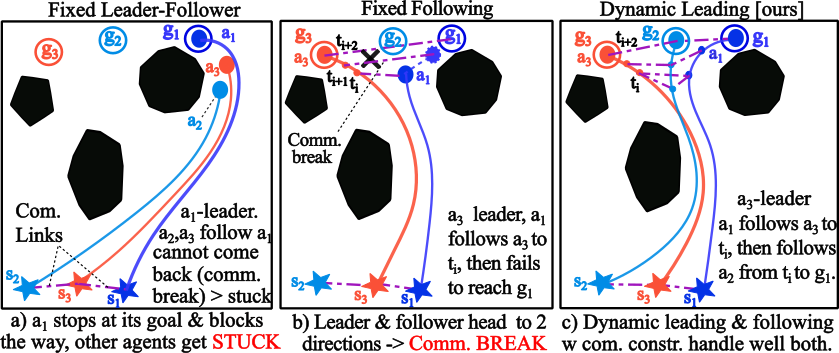
\includegraphics[width=1.0\columnwidth]{intro_fig1.png}
    \caption{\textbf{Fixed leader-follower approaches fail in scenarios a) \& b). Our framework, MA-DL, can handle both (c).} If $a_1$'s leading causes the team to get stuck (a), \textit{dynamic leading} allows another agent take over as the new leader. When the leader and follower move to different directions (b), followers are allowed to pursue another agent to its goal. 
    }
    \label{fig:Intro}
\end{figure}

To address these challenges, this work develops a framework for solving multi-agent pathfinding problem with limited communication range (MALCR), ensuring a connected communication channel in the team at any time. 
We propose a novel technique: \textit{dynamic leading} which allows any agent to become the new leader during multi-agent tree expansion, allowing planning to further expand the multi-agent tree if the current leader cannot make progress. Once the leader agent has planned, follower agents plan, ensuring that the resulting path is always in communication to at least one agent.
% so as to maintain 
%. This technique helps the team move forward if the current leader does not make progress.
% OLD VERSION: We propose a novel technique: \textit{dynamic leading} which allows any agent to become the new leader during motion tree expansion if it goes farther than the current leader. This technique helps the team move forward if the current leader does not make progress.We also allow the followers planning without a fixed following scheme as long as it ensures a communication link to at least one agent.

We introduce an algorithm for planning in multi-agent systems with communication distance constraints: MA-DL. 
The experiments show that our framework results in fast and effective planning, handling up to 25 agents with more than 90\% success-rate across five environment types where baselines, centralized planning with composite states and platooning leader-follower approach, routinely fail. 

% Experimentally, our framework results in fast and effective planning, outperforming two standard baselines: centralized planning with composite states and platooning leader-follower approach.
% \textbf{[TODO: update this with some actual numbers.]}

\begin{figure*}[ht]
\centering
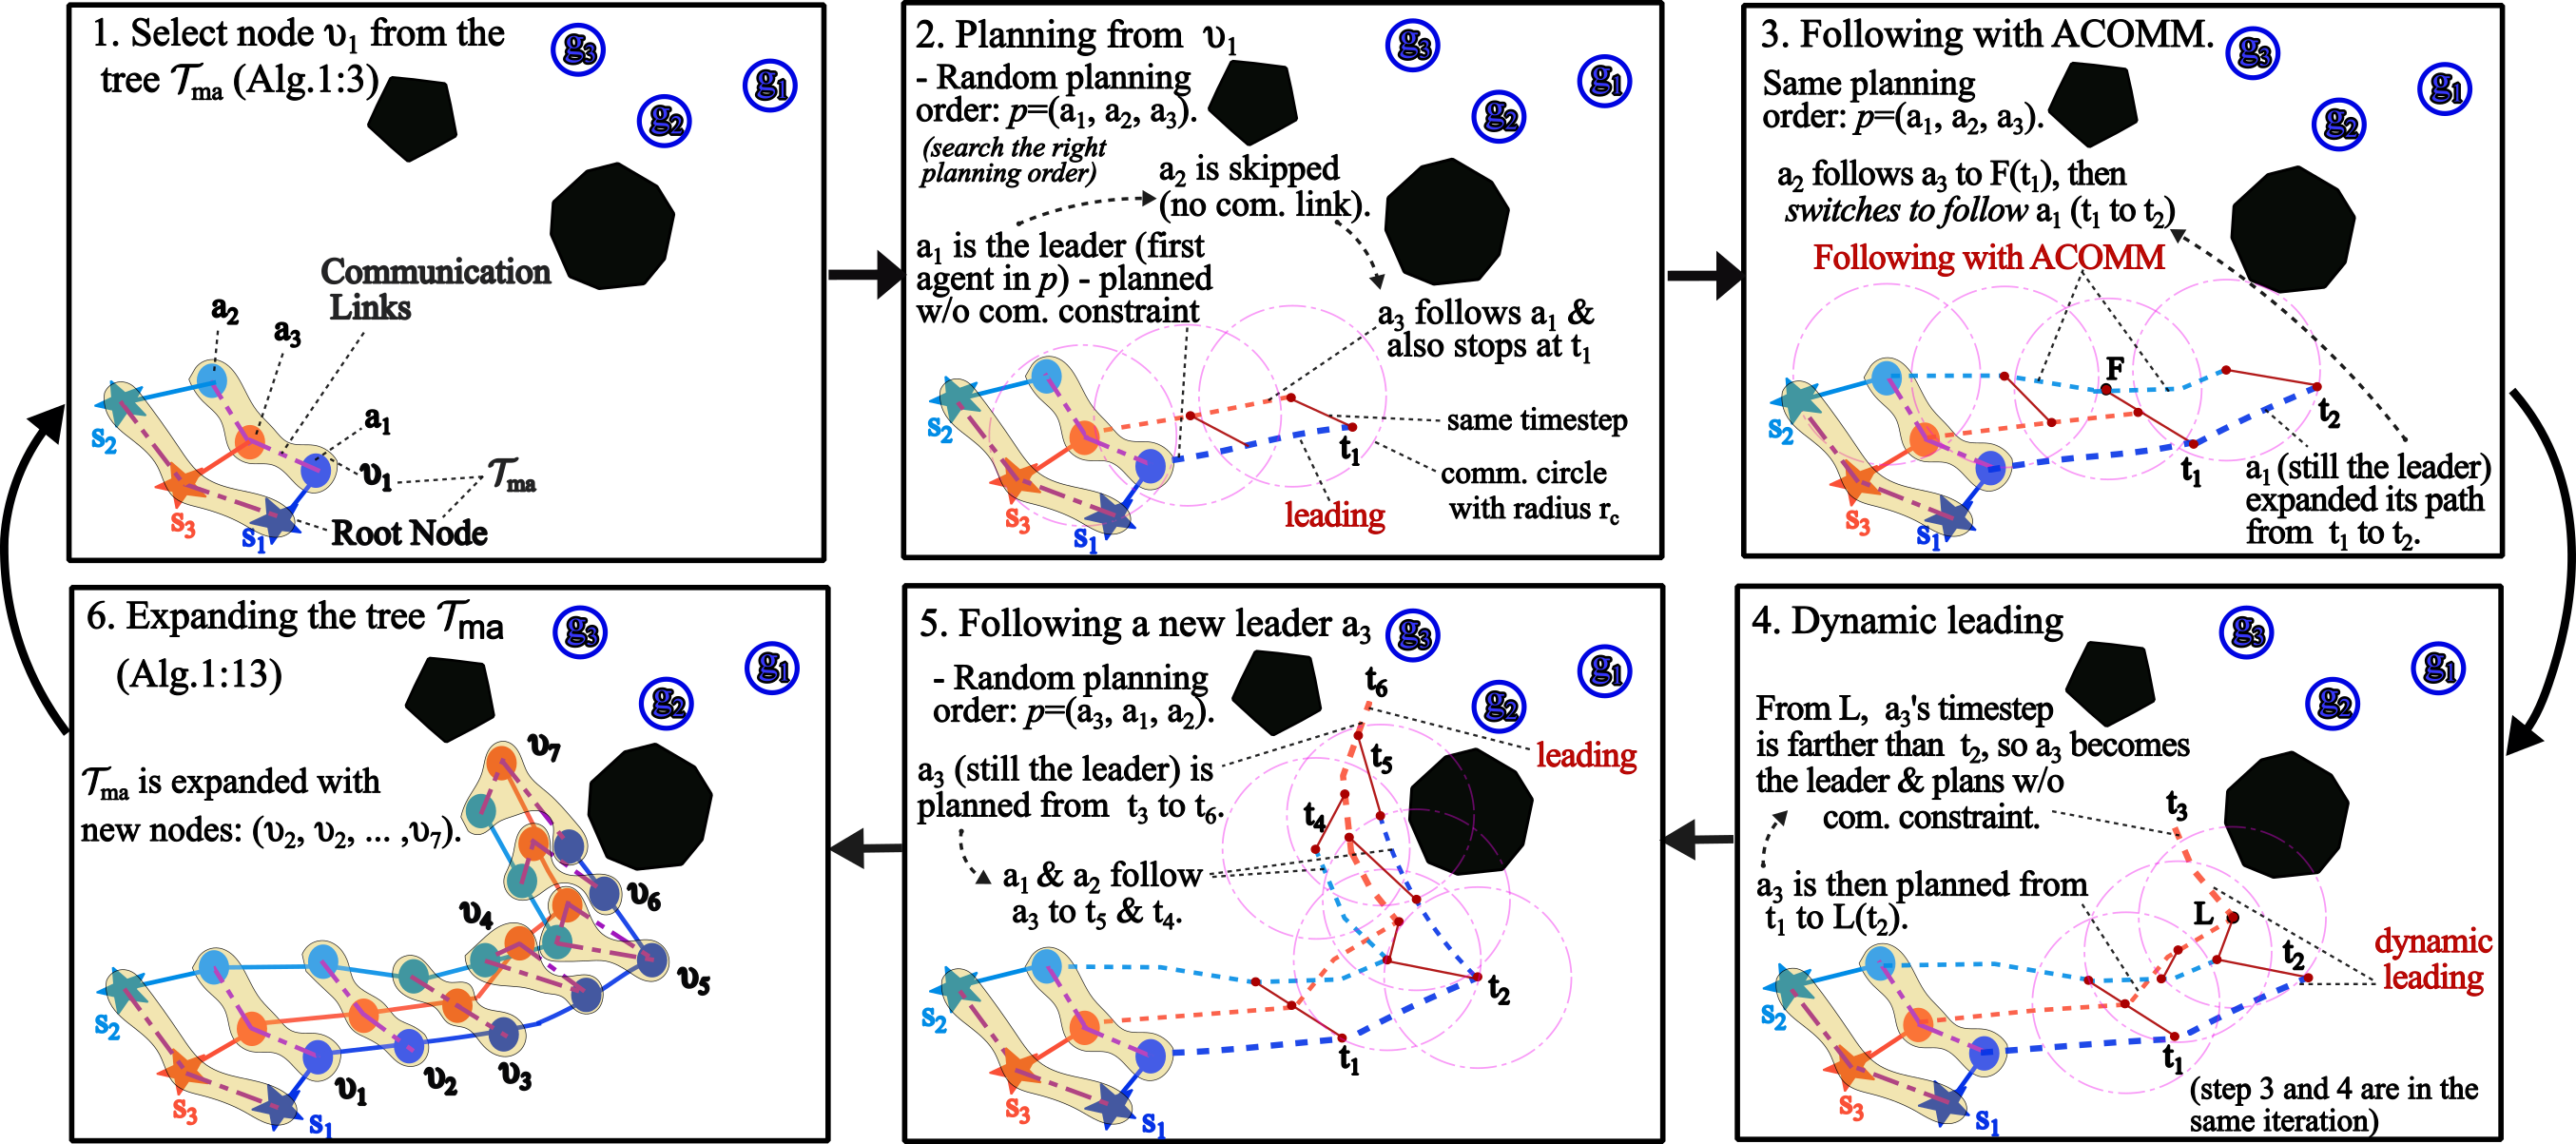
\includegraphics[width=0.95\textwidth]{fw_ver3.png}
\caption{\textbf{An illustration of one step expanding the MATree with 3 agents}. $a_1$, $a_2$, and $a_3$, start at $s_1$, $s_2$, and $s_3$, aiming for their goals $g_1$, $g_2$, and $g_3$ while avoiding the obstacles (black) and other agents. From node $v_1$ in the multi-agent tree $\Tree_{ma}$ (step 1), the planner implements single plannings with random planning order (step 2--5), then expand $\Tree_{ma}$ based on the paths found (step 6). In step 3, $a_2$ follows $a_3$ to maintain communication links. At $t_1$(F), when $a_3$ stops, $a_2$ switches to follow $a_1$. Our key contribution, \textit{dynamic leading}, occurs at step 4 when $a_3$ follows $a_2$ to $t_2$ (L), then becomes the new leader and plan to $t_3$. In the next iteration, other agents follows $a_3$ before expanding the MATree in step 6.}
\label{fig:fw}
\end{figure*}


\section{Related Work} \label{sec:related-work}
% Finding paths for a fleet of agents while maintaining connection among the agents is an active research problem in the field of artificial intelligence. There are several approaches possible to solve the MALCR problem.

There exist multiple approaches that seek to solve multi-agent path finding problems, 
in the absence of a communication constraint, that could in theory be adapted to solve the MALCR problem.
% have applicability to solving our problem.
To effectively scale to more agents, approaches in this space are typically designed around 
reducing the exponential growth of the planning tree with planning time horizon.
Wagner and Choset \cite{wagner2015subdimensional} proposed M$^*$ algorithm, which plans individually 
for each agent, yet builds composite states for agents and expands the local planning tree when their paths are in collision.
% which only builds composite states for agents if their paths are in collision; while it plans individually for other agents. 
Though M$^*$ works well if the agents are far apart, when agents are close to each other, 
collisions occurs frequently, causing the planning joint-state increases rapidly until fully incooperating of all agents and limiting 
its efficacy for solving our limited-communication problem, which requires that agents be near to one another. 
Solovey, Salzman, and Halperin \cite{solovey2016finding} introduced the dRRT planner, which uses 
a implicit composite roadmap---a product of single-agent roadmaps. Their algorithm grows a multi-agent 
tree in this composite roadmap using RRT. However, using such a roadmap requires abstracting low-level 
details of each robot's motion over time, making it difficult to apply their approach for planning with communication constraints.
% Okumura et al. \cite{okumura2023offline,okumura2022priority} proposed a priority-based approach PIBT to solve the multi-agent path finding problem.
PIBT~\cite{okumura2022priority} and BMAA*~\cite{sigurdson2018multi} expand a single action for each agent 
in each planning iteration. These planners can handle well deadlocks among the agents. However, 
there are two issues for these planners to solve MALCR problem. The first one is their short-term action 
selection strategy, which can result in situations where followers are unable to find actions that keep them 
within the leader's communication range. The second one is their fixed planning order causing followers fail to 
plan when their initial positions are out of the leader's communication range (Fig.~\ref{fig:Intro}b).
% The first is their short-term selecting action strategy which would lead to situations on which followers cannot find actions to follow leader within communication range.
% Moreover, their fixed planning order makes followers fail to move because their initial positions are out of communication with their leader .
Okumuar et al.~\cite{okumura2023offline} proposed the OTIMAPP planner which employs Deadlock-based 
Search (DBS) to resolve conflict among paths determined through prioritized planning. 
In addition to the limitation of a fixed planning order (as mentioned above), OTIMAPP requires 
a new technique to modify the computed paths while adhering to deadlock and communication constraints.
In general, it is very challenging to adapt these approaches to solve the MALCR problem
in which each member of the team must be in constant communication with one another in continuous time. 

Specific to the MALCR problem, \emph{platooning} has emerged as a state-of-the-art solution for multi-agent 
path finding in which the motion of a leader-agent is planned first and follower-agents planned one at a time 
in sequence to follow the agent that proceeded them, and so is designed to maintain communication constraints between pairs of agents.
% The second approach is platooning--state-of-the-art method--to solve MALCR problem. In this approach, there is one leader and multiple followers in the team.
% A following agent needs to follow its preceding agent or the leader based on its order on the team, with the assumption that all agents are moving to the same direction. 
Most existing work in platooning performs full motion planning only for the leader, and uses a low-level 
controller to regulate followers to maintain a distance from the preceding agents~\cite{shojaei2019tracking,huang2019platoon}.
% \citet{shojaei2019tracking} and \citet{huang2019platoon} proposed a two layer control framework to regulate the followers pursuing the preceding vehicles. The higher level manages the path following, and the lower level deals with the vehicle's dynamics.
Qian et al. \cite{qian2016mpcautonomousvehicles}, Zhao et al.~\cite{zhao2017design}, and Gao et al.~\cite{gao2019multilane} 
introduced model predictive controller that generate trajectories for a virtual center, which followers need to track.
% The following is regulated by model predictive control.
% If a vehicle leaves the team, its followers are reassigned to its preceding vehicle.

However, recent work in the space of conflict-based search (CBS)~\cite{ma2019searching} 
has proven that planning with a fixed vehicle order in general, including platooning, 
is incomplete and frequently becomes stuck when the leader moves in a direction different 
to the follower's goals, as we show in Fig.~\ref{fig:Intro}, or when the team must shuffle 
their planning order during travel to reach their goals without violating communication constraints.
Overcoming this limitation in general requires a planner that allows for \emph{dynamic leading}, 
in which the leader can change during multi-agent tree expansion when the team fails to make progress towards the goal.


% Overcoming this limitation requires a planning that allows a dynamic 
% However, methods, like platooning, that assume a fixed vehicle or planning order can become stuck~\cite{ma2019searching}, particularly when 
% those methods with fixed planning order struggle to handle scenarios where the leader stalls or moves in a direction different to the followers' goals. 
% To overcome these issues, we need a dynamic leading and ordering strategy to change the leader as the team does not make progress. 

\section{Problem Definition} \label{sec:problem-formulation}

We formally define the Multi-Agent Path Finding with Limited Communication Range (MALCR) problem as follows.
There are $n$ agents $\{a_1, \ldots, a_n\}$ and a known world $\World$ with obstacles $\Obstacle = \{\Obstacle_1, \ldots, \Obstacle_m\}$. 
The agents start at the initial positions $s^\Var{init} = \Pair{s^\Var{init}_1, \ldots,s^\Var{init}_n}$ and 
head to the goals $\GoalPos = \{\GoalPos_1, \ldots,\GoalPos_n\}$, where $s_i, g_i \in \World$ and $s_i, g_i \notin \Obstacle$. 
The initial positions and goals are chosen so as to satisfy the team communication constraint, formally defined below.
% At the initial positions and goals, the agent team maintain constant team communication.

The world $\World$ is divided into sub-divisions $\Subdiv$, which are obstacle-free regions. 
A graph $\mathcal{G}$ is created where the vertices are the centroids of $\Subdiv$ and the edges represent connections 
of neighboring sub-divisions. 
An agent moves to a neighboring sub-division with constant velocity $\Var{v}_c$ by taking the 
action: \textit{Move}$(v,u)$, where $v,u$ are neighbor vertices in $\mathcal{G}$. 
% To check for collisions or communication among agents, the action is considered as a sequence of jumps with small 
% distance between the sequential points along the line $l_{vu}$. 
As reaching its goal, the agent takes the action of \textit{Stop} = \textit{Move}$(v,v)$. Agents moving over 
$\mathcal{G}$ are guaranteed to be \textit{collision-free} with respect to the static obstacles. 
Time and agents' positions are continuous due to varied lengths of actions.

We define two levels of communication constraint for the agents. 
The first level is between two agents, referred to as \textbf{agent communication constraint} (ACOMM), 
which requires the distance between their positions to be less than 
or equal to the communication range $r_c$.
The second level applies to the entire agent team, referred to 
as \textbf{team communication constraint} (TCOMM), which requires 
the team to form a spanning tree where the edges represent the 
connections between pairs of agents satisfying the ACOMM constraint.
% When we refer to \textit{communication constraint} in general, we mean the TCOMM constraint.
An action \textit{Move($v,u$)} satisfies the \textit{ACOMM constraint} 
if during the movement \textit{Move($v,u$)} the agent has at least one 
neighboring agent within a distance of $r_c$.
% throughout the segmented points on along the line $l_{vu}$ connecting the node $v$, at each point the agent has at least one neighboring agent within distance of $r_c$.
% The cost of an action is the traveled distance between the agent's current position and the destination vertex.

% As agents move along the edges in $\mathcal{G}$, there is no collision between agents and static obstacles. Therefore, 
A \textbf{collision} occurs between two agents, $a_i$ and $a_j$, when their distance is less than a threshold $d_c$ at timestep $t$. 
A \textbf{path} is a sequence of waypoints to transition an agent from a position $p_s$ to position $p_g$ with constant velocity $\emph{v}_c$. We say a path is \textbf{reach-goal} if it can lead the agent to the goal, is collision-free, and the movement between two sequential waypoints satisfies ACOMM constraint;
When an agent stops at its goal, we still consider collision and ACOMM constraints. 
A path is \textbf{valid} if it is \emph{reach-goal} and at the goal $p_g$ from $t_g$, the agent's action \textit{Stop} still satisfies ACOMM and is collision-free.
% The cost of a path is the sum of Euclidean distances between the sequential waypoints on the path.

The objective is to compute \textit{valid} paths $\{\Traj_1, \ldots, \Traj_n\}$, one for each agent, so that $\Traj_i$ starts at $s^\Var{init}_i$, reaches $\GoalPos_i$, and the agents satisfy TCOMM constraints from the start time to the time the last agent reaches its goal. 
We develop a MAPF framework that seeks to reduce the overall planning time and the travel distances.

% \begin{algorithmic}[1][ht]
\begin{algorithm}[ht]
\caption{\Function{MA-DL} module}
\label{alg:MADIST}
\footnotesize
% \setstretch{1.5}
\begin{algorithmic}
\STATE \text{INPUT}: $n$: \text{number of agents}, $g=\{g_1,...,g_n\}$: goals, $\World$: \Var{world}, $s^\Var{init}=\{s_1^\Var{init},...,s_n^\Var{init}\}$: \text{starts}, $t_\Var{ds}$: \text{max runtime}
\STATE \text{OUTPUT: paths} $\Traj=\{\Traj_1,...,\Traj_\Var{n}\}$
\end{algorithmic}
% \newline
\begin{algorithmic}[1]
% \setstretch{1.1}
% \STATE \hrulefill
% \STATE \rule{\textwidth}{0.5pt}
\STATE $\Tree_\Var{ma}\!\gets \Function{InitMATree}(s^\Var{init}, t=0)$;
$\Subdiv \! \gets\!\Function{SubDivision}(\World)$; $\mathcal{G} \gets \Function{CreateGraph}(\Subdiv, g)$\;
\STATE $\mathcal{H} \gets \{\Function{CalHeursitic}(\mathcal{G}, g_1),\ldots, \Function{CalHeursitic}(\mathcal{G}, g_n)$\}\;
\WHILE{$ \Function{time}() < t_\Var{ds}$}
    \STATE $v \gets \Function{SelectNode}(\Tree_\Var{ma})$; $p \gets \Function{InitOrder}(v)$; $\Traj^s \gets \Function{InitPaths}(v)$\;
    \STATE \textbf{if} ($v.\Var{visited}$) \textbf{then} $\Function{Shuffle}(p)$\;
    \FOR{$ 1 \leq k \leq m $}
        \STATE $\Var{allRG} \gets \True$; \textbf{if} $k>m_t$ \textbf{then} $\Function{Shuffle}(p)$\;
        \FOR{$1 \leq i \leq n$}
            \STATE \textbf{if } $\Function{FoundGoal}(\Traj^s_{p_i})$ \textbf{then continue}\;
            \STATE $\Traj^t\!\gets\!\Function{SAPF}(p_i, g_{p_i}, \Traj^s, \mathcal{G}, \mathcal{H}_i)$; $\Traj^s_{p_i}.\Function{Insert}(\Traj^t)$\; 
            \STATE \textbf{if} $\Function{FoundGoal}(\Traj^s_{p_i})$ \textbf{then} $\Function{ModifyIfOverlap}(p_i, \Traj^s, \Var{allRG})$\;
            \STATE \textbf{else} $\Var{allRG}=\False$\; 
        \ENDFOR
        \STATE \textbf{if} $\Var{allRG}$ \textbf{then break}\;
    \ENDFOR
    \STATE $\Function{ExpandMATree}(\Tree_\Var{ma}, \Traj^s, v)$; $v.\Var{visited} \gets \True$\;
    \STATE \textbf{if} $\Var{allRG}$ \textbf{then break};
\ENDWHILE

\STATE $\Var{vid} = \Function{ClosestNodeToGoal}(\Tree_\Var{ma})$\;
\STATE \textbf{return} $\Function{GetPaths}(\Tree_\Var{ma}(\Var{vid}))$\;
\end{algorithmic}
\end{algorithm}


\section{Methods} \label{sec:methods}

\begin{algorithm}[ht]
\caption{\Function{SAPF} module}
\label{alg:sapf}
\footnotesize
\begin{algorithmic}
\STATE \text{INPUT}: $\rho$: \text{agent's ID}, $g_\rho$: goal, $\mathcal{G}$: init. graph, $\Traj^s$: \text{previous planned paths}, 
$t_\Var{sa}$: \text{max runtime}, $\mathcal{H}_\rho$: \text{shortest path heuristic}
\STATE \text{OUTPUT}: a path $\Traj_\rho$
\end{algorithmic}
% \newline
% \hrule
\begin{algorithmic}[1]
\STATE { $\mathcal{G}^s = \Function{AddNodes}( \mathcal{G}, g_\rho, \Traj^s_\rho.\Var{end})$\; }
% $\Function{CalculateHeursitic}(\mathcal{G}^s, g_\rho)$\;}
\STATE $v_g\!\gets\! \Function{GetNode}(g_\rho,\mathcal{G}^s)$; 
$v_s\!\gets\!\Function{GetNode}(\Traj^s_\rho.\Var{end}, \mathcal{G}^s)$\;
\STATE $\Var{openList}.\Function{Add}(v_s)$; $\Var{closedSet} \gets \{\}$; $v_\Var{best} \gets v_s$\;

\WHILE{$\Var{openList}$ \textbf{not empty} \textbf{and} $\Function{time}() < \Var{t}_\Var{sa}$}
    \STATE $v \leftarrow \Var{openList}.\Function{Pop}()$; $\Var{closedSet}.\Function{Add}(v)$\;
    \STATE \textbf{if} $v = v_g$ \textbf{then return} $\Function{getpath}(v_s, v,\mathcal{G}^s)$ \;
    \FOR{$u$ \textbf{in} $\Function{GetNeighbors}(v)$}
        \IF{$u  \textbf{ is not in }  \Var{closedSet}$}
            \STATE $u.\Var{parent} \gets v$; $d_{uv} \gets \Function{Distance}(v, u)$; $u.g \leftarrow v.g$ + $d_{uv}$\;
            \STATE $u.t \gets v.t$ + $d_{uv}/\text{v}_c$; $u.h \gets \Function{GetHeuristic}(u, \mathcal{H}_\rho)$; $u.f=u.g+u.h$\;
            \IF{$\Function{IsNodeValid}$($\rho, \Traj^s, u, v, r_c)$}
                \STATE $\Var{openList}.\Function{Add}(u)$\;
                \STATE \textbf{if} $u = v_g$ \textbf{then return} $\Function{GetPath}(v_s,u,\mathcal{G}^s)$\;
            \ENDIF
        \ELSIF{$v.g +d_{uv} < u.g$}
            \STATE $u_1 \gets \Function{Copy}(u)$; $u_1.t \gets v.t+d_{uv}/\text{v}_c$\;
            \IF{$\Function{IsNodeValid}$($\rho, \Traj^s, u_1, v, r_c$)}
                \STATE $u.\Var{parent} \gets v$; $u.t \leftarrow v.t+d_{uv}/\text{v}_c$;
                $u.g \gets v.g+d_{uv}$; $u.f=u.g+u.h$\;
            \ENDIF
        \ENDIF
        \STATE \textbf{if} $v_\Var{best}.f > u.f$ \textbf{then} {$v_\Var{best} \gets u$}\;
    \ENDFOR
\ENDWHILE
\STATE \textbf{return} $\Function{GetPath}(v_s, v_\Var{best},\mathcal{G}^s)$\;
\end{algorithmic}
\end{algorithm}

% In this section, we present our work to solve the MALCR problem. 
Our framework, named as \emph{MA-DL}, consists of two modules: Multi-agent Path Finding with Dynamic Leading (MA-DL) and Single-Agent Path Finding (SAPF).

\textit{High Level Overview}:
The main loop of the \emph{MA-DL} module (Alg.~\ref{alg:MADIST}) expands a multi-agent (MA) 
planning tree $\Tree_{ma}$ whose growth is illustrated in Fig.~\ref{fig:fw}. The MA tree is used 
to represent motion expansion of all agents. Its role is to keep track of planning progress 
for all agents, and the node with lowest value of cost and heuristic will be selected to 
expand in the next iteration.
To ensure all nodes in $\Tree_{ma}$ have a chance of being selected, their costs are 
penalized after each selection.
% Starting from node $v_1$ (Fig.~\ref{fig:fw}.1), 
The MA tree expansion occurs in a loop (Fig.~\ref{fig:fw}:2--5), in which each 
agent's path is expanded in order. 
The single-agent planner (SAPF, Alg.~\ref{alg:sapf}) finds \textit{reach-goal} shortest 
paths for the agents one by one according to the planning order $p$, such that each agent
maintains communication with at least one of the agents that plans before it.
Difference to prioritized planning approach~\cite{van2005prioritized} with fixed leading, 
the leader agent in our planner is dynamic: through dynamic leading technique 
(Alg.~\ref{alg:isNodeValid}) which allows any agent take the leading role if it goes 
further than other agents, or shuffling the planning 
order whenener planning cannot further expand the multi-agent tree (Alg.~\ref{alg:MADIST}:6).
% However, our planning order is dynamic: though a heuristic is used to select an initial 
% planning order $p$ (Alg.~\ref{alg:MADIST}:3), this order is shuffled whenever planning 
% cannot further expand the multi-agent tree (Alg.~\ref{alg:MADIST}:6).
After each planning loop, the multi-agent tree is expanded with new nodes built from the individual paths (Fig.~\ref{fig:fw}.6).
Our \textit{dynamic leading} technique (Fig.~\ref{fig:fw}.4) allows the MA-DL planner 
to handle the challenging situations in Fig.~\ref{fig:Intro}.


\subsection{MA-DL MODULE} \label{sec:MADIST}
This module manages the multi-agent tree (MATree) $\Tree_{ma}$, selects nodes to expand, 
dynamically selects planning orders, and triggers single-agent plannings. 
% If an agent finds a \textit{reach-goal} path, the module checks whether it is \textit{valid}. The path is invalid if the \textit{Stop} action at the goal at time $t$ blocks the future movement of earlier planned agent (according to planning order $p$). The situation is called \textit{collision-at-goal} in \cite{bui2024multi} and can be resolved by modifying the earlier planned paths if they go through the goal after $t$. 
% After the single plannings are finished, the tree $\Tree_{ma}$ is then expanded. The main loop breaks if all agents find their \textit{valid} paths or the runtime is up.

The module gets the number of agents $n$, the goals $g$, initial start $s^\text{init}$, 
and the world $\World$ as inputs and returns the \textit{valid} paths or, if valid paths 
cannot be found, those closest to the goal. 
The algorithm (Alg.~\ref{alg:MADIST}) starts by initializing a multi-agent tree 
$\Tree_{ma}$ with the root consisting of all initial positions $s^\text{init}$ 
(Alg.~\ref{alg:MADIST}:1). 
The world $\World$ is divided into sub-divisions $\Subdiv$ of a predefined area, with 
obstacle-overlapping sub-divisions further subdivided 
along their largest dimension until they clear or reach a size threshold.
A graph $\mathcal{G}$ is created from the centroids of the obstacle-free sub-divisions, 
while the edges represent the  
connections between neighboring sub-divisions (sharing boundaries or corners).
We compute the shortest paths $\mathcal{H}$ from all sub-divisions to the agent goals $g$ 
as heuristics by the function $\Function{CalHeuristic()}$ (Alg.~\ref{alg:MADIST}:2).
In the main loop (Alg.~\ref{alg:MADIST}:3--15), a node $v$ with smallest cost 
(defined at Alg.~\ref{alg:ExpandMATree}.14) is selected from $\Tree_{ma}$. The cost of $v$ is 
then increased to encourage selecting other nodes.
A heuristic function $\Function{INITORDER()}$ returns an initial planning order $p$. 
A list of $n$ paths $\Traj^s$ is initialized from $v$ (Alg.~\ref{alg:MADIST}:4). 
If the node $v$ is visited, the planning order \emph{p} is shuffled to get a different 
planning order (Alg.~\ref{alg:MADIST}:5).
% As the runtime $t_{ds}$ is large enough, we surely can attempt all planning orders at $v$. 
The planning loop (Alg.~\ref{alg:MADIST}:6--13) attempts to find valid paths 
for the agents.
The loop starts by setting the variable $\Var{allRG}$ to $\True$ (Alg.~\ref{alg:MADIST}:7).
The planning order \emph{p} is shuffled after $m_t$ iterations of failing to 
reach the goal (Alg.~\ref{alg:MADIST}:7). 
The \emph{for} loop (Alg.~\ref{alg:MADIST}:8--12) plans for each agent in order 
by calling the module $\Function{SAPF}$ and then the returned paths is inserted 
into $\Traj^s_{p_i}$ (Alg.~\ref{alg:MADIST}:10). If $\Traj^s_{p_i}$ is \textit{reach-goal},
it is then checked for validity (\textit{valid}) by the function $\Function{MODIFYIFOVERLAP}()$. 
The path is invalid if the \textit{Stop} action at the goal at time $t$ blocks 
the future movement of an already-planned agent (according to planning order $p$), 
a situation called \textit{collision-at-goal} by Bui et al.~\cite{bui2024multi}.
If the situation occurs, the function modifies the earlier planned paths and 
set $\Var{allRG}$ to $\False$ (Alg.~\ref{alg:MADIST}:11). 
If the path is not reach-goal, $\Var{allRG}$ is set to $\False$~(Alg.\ref{alg:MADIST}:12). 

After all agent planning has completed, the function $\Function{EXPANDMATREE()}$ is 
triggered to expand $\Tree_{ma}$ from $v$ using the agent's paths $\Traj^s$ 
(Alg.~\ref{alg:MADIST}:14); then the node $v$ is also marked as \textit{visited}.
If all agents reach the goals ($\Var{allRG}$ is still $\True$), we break the 
\emph{while} loop (Alg.~\ref{alg:MADIST}:15), then return paths for all agents 
from $\Tree_{ma}$ (Alg.~\ref{alg:MADIST}:16--17).

\begin{algorithm}[ht]
\caption{$\Function{IsNodeValid}(\rho, \Traj^s, u, v, r_c$) (\textit{Dynamic leading is employed}) }
\label{alg:isNodeValid}
\begin{algorithmic}[1]
\footnotesize
\STATE $\Var{lead} \leftarrow \True$; $\Var{comm} \leftarrow \False$\;
    \FOR{ $1 \leq i \leq |\Traj^s |$ }
        \STATE \textbf{if} $u.t \leq \Traj^s_i.\text{maxtime}$ \textbf{then} $\Var{lead} \gets \False$
    \ENDFOR
    \STATE \textbf{if } \text{lead} \textbf{then} $\text{lead} \gets \Function{IsCOMMAtGoal}(u, \Traj^s, \rho)$\;
    \FOR{$1 \leq i \leq |\Traj^s|$}
        \STATE \textbf{if} $\Function{IsCollision}(u, v, \Traj^s_i, \rho)$ \textbf{then return} $\False$\;
        \STATE \textbf{if} $\Function{IsCOMMS}(u, v, \Traj^s_i, \rho, r_c)$ \textbf{then} $\Var{comm} \leftarrow \True$\;
    \ENDFOR
    \STATE \textbf{return} {$(\Var{lead} \ \| \ \Var{comm})$ }\;
\end{algorithmic}
\end{algorithm}

\subsection{SAPF MODULE}\label{sec:SAPF}
Single-Agent Path Finding (SAPF) finds a shortest \textit{reach-goal} path for an agent. 
This planner searches actions on $\mathcal{G}$ that satisfy the ACOMM constraint and 
are collision-free. With enough runtime, the planner can explore all possible paths 
and so is probabilistically complete.
If it fails, it returns the closest-to-goal path. Agents are assumed to have the same 
velocity $\Var{v}_c$.
The inputs are the agent's ID $\rho$, goal position $g_\rho$, a graph of the world 
sub-divisions $\mathcal{G}$, planned paths of previous agents $\Traj^s$, and the shortest
path to the goal heuristic $\mathcal{H}$.

To initialize, a new graph $\mathcal{G}^s$ is created by adding to $\mathcal{G}$: 
(i) the current agent position $\Traj^s_\rho.\Var{end}$ and (ii) the goal $g_\rho$, 
each of which connect to the centroid of the sub-division to which they belong (Alg.~\ref{alg:sapf}:1).
% then, the function $\Function{CalculateHeuristic}()$ is called to calculate shortest 
% paths from any vertex in $\mathcal{G}^s$ to $g_\rho$ by Dijkstra's algorithm 
% , used as heuristics to guide the planner.
The variables $v_g$ and $v_s$ are the goal and current nodes (Alg.~\ref{alg:sapf}:2).
$v_s$ is then added into $\Var{openList}$---a priority queue data structure, which 
sorts its elements by their cost-to-goal. \text{closedSet} and the closest-to-goal 
node $v_\text{best}$ are also initialized (Alg.~\ref{alg:sapf}:3).

The search loop (Alg.~\ref{alg:sapf}:4--18) is: a node with lowest cost is popped 
out from $\Var{openList}$ (Alg.~\ref{alg:sapf}:5); then we iterate through all its 
neighbors (Alg.~\ref{alg:sapf}:7--18) to find valid nodes, calculate or update their 
costs, parents, and timestep, then add them into openList.

\begin{figure}[b]
    \centering
    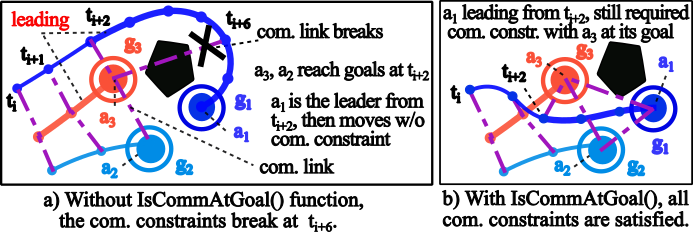
\includegraphics[width=0.9\columnwidth]{outComAtGoal_2.png}
    \caption{\textbf{Out-of-communication-at-goal situation (a) and how \Function{ISCOMMATGOAL}() works (b).} In both situations, the planning order is ($a_3, a_2, a_1$) and the leader is changed at $t_{i+2}$.
    }
    \label{fig:outComAtGoal}
\end{figure}

For a node $u$ to be valid, the move action from its parent $v$ must be collision-free 
and satisfy the ACOMM constraint. Both of these requirements are checked by the 
function $\Function{ISNODEVALID}()$ (Alg.~\ref{alg:sapf}:11,16). 

\begin{algorithm}[ht]
\caption{$\Function{ExpandMATree}(\Tree_\Var{ma}, \Traj^s, v$) }
\label{alg:ExpandMATree}
\begin{algorithmic}[1]
\footnotesize
\STATE $v_p \gets v$; $\Var{timeList} \gets \{ \} $ \CodeComment{priority queue}\;
\FOR{$0 \leq $ i $ < | \Traj^s|$ }
    \STATE \textbf{for} $0 \leq $ j $ < | \Traj^s_i.\Var{times} |$ \textbf{do} \Var{timeList}.$\Function{Insert}(\Traj^s_i.\Var{times} [j])$ \;
\ENDFOR
\FOR {$t$ \textbf{in} \Var{timeList} }
    \STATE $v_n \leftarrow \Function{NewNode}()$; $v_n(\Var{parent}, g,t) \leftarrow (v_p,v_p.g,t)$\;
    \FOR{$0 \leq j < | \Traj^s|$} 
        \STATE \textbf{if } $t > \Traj^s_j.\Var{end}.t$ \textbf{then}\;
        \STATE \quad \textbf{if } $\Function{FoundGoal}(\Traj^s_j)$  \textbf{then} $\Var{pos} \leftarrow \Traj_j.\Var{end.pos}$\;
        \STATE \quad \textbf{else return}\;
        \STATE \textbf{else} $\Var{pos} \leftarrow \Function{GetPosAtTime}(\Traj^s_j, t)$ \;
        \STATE $v_n.\Var{state}.\Function{Insert}(\Var{pos}) $; $d = \Function{Dist}(v_p.\Var{state}_j, v_n.\Var{state}_j)$\;
        \STATE $v_n.g$ += $d$; $\Traj^s_j$.\Var{costogoal} -= $d$;
        $v_n.h$ += $\Traj^s_j$.\Var{costogoal}\;
    \ENDFOR
    \STATE $v_n.f \gets v_n.g$ + $v_n.h$\;
    \STATE $\Tree_\Var{ma}.\Function{Append}(v_n)$; $v_p \gets v_n$\;
\ENDFOR
\end{algorithmic}
\end{algorithm}

\paragraph{\textbf{IsNodeValid}() Function}

This function (Alg.~\ref{alg:isNodeValid}) checks the validity of action $\textit{Move}(v,u)$ for an agent $\rho$ starting at timestep $v.t$.
For agent-collision detection, $\Function{IsCollision}()$ (Alg.~\ref{alg:isNodeValid}:6) checks if any segmented point along the line $l_{vu}$ (connecting $v$ and $u$) collides with the planned paths in $\Traj^s$ (Alg.~\ref{alg:isNodeValid}:5) at corresponding timesteps. If a collision occurs, the node is invalid. 

The ACOMM constraint check depends on whether agent $\rho$ is a leader or follower. In our approach, an agent becomes the new leader if its timestep during expansion is ahead of all others (Alg.~\ref{alg:isNodeValid}:2--3); we call this \textit{dynamic leading}.
Because it plans farther out in time than other agents, the leader is not subject to any communication constraints when expanding its plan.
A follower agent $\rho$ must satisfy the ACOMM communication constraint: that it must maintain communication with another agent while moving. 
The function $\Function{ISCOMMS}()$ (Alg.~\ref{alg:isNodeValid}:7) checks that agent $\rho$ can communicate with a neighbor during its action. 

During \textit{dynamic leading}, a situation called \textit{out-of-communication-at-goal} can occur, which is shown in Fig.~\ref{fig:outComAtGoal}. To prevent this situation, we propose the function $\Function{IsCommAtGoal}$().


% \paragraph{\Function{IsComAtGoal()} Function}
\paragraph{\textbf{IsCommAtGoal}() Function}
In Fig.~\ref{fig:outComAtGoal}, at $t_i$ agent $a_3$ is the leader, and reaches its goal in two steps ($t_{i+1}$ and $t_{i+2}$). $a_2$ follows $a_3$ and also stops at its goal by $t_{i+2}$.
Agent $a_1$ follows $a_3$ until $t_{i+2}$, and then becomes the leader, planning without ACOMM constraints shown in Fig.~\ref{fig:outComAtGoal}.a. However, the MATree $\Tree_{ma}$ expansion halts at $t_{i+6}$ due to communication breakdown. 
The function $\Function{ISCOMMATGOAL}()$ guides $a_1$ to remain in communication. It is triggered when the leader is changed (Alg.~\ref{alg:isNodeValid}.4). It checks if any of the new leader's neighbors have reached their destination. If so, the leader's action $\textit{Move}(v,u)$ must meet the ACOMM constraint with an at-goal agent. If it cannot, its leader status is revoked.

% neighbor (at the goal) of the new leader has reached its destination. If so, the leader's action $\textit{Move}(v,u)$ must meet the ACOMM constraint with the at-goal agents. If not, its leader status is revoked.

\subsection{EXPAND MULTI-AGENT TREE}
Function $\Function{ExpandMATree}()$ (Alg.~\ref{alg:ExpandMATree}) integrates the paths from the single agents $\Traj^s$ and adds the combined paths to expand the multi-agent tree $\Tree_\Var{ma}$.
% Function $\Function{ExpandMATree}()$ (Alg.~\ref{alg:ExpandMATree}) expands the tree $\Tree_\Var{ma}$ along the single paths $\Traj^s$. If agents reach goals, the goals are their current positions.
Each node on $\Tree_{ma}$ has an associated timestep and the agent positions are interpolated to make them match for each single agent path.
% along the single paths for each timestep, which are different along the agent's paths.
% With different timesteps , all agents' positions must be at the same timestep. The agents move on continuous time and coordination, thus their timesteps on the paths are different. So, the agent positions are interpolated by timesteps. 
% The heuristic value of $v_n$ is the sum of remaining cost-to-goal of the single paths.

The \emph{for} loop (Alg.~\ref{alg:ExpandMATree}:2--3) collects all timesteps of the waypoints on the single paths and inserts into a priority queue $\Var{timeList}$. 
The second \emph{for} loop (Alg.~\ref{alg:ExpandMATree}:4--14) goes through all elements in $\Var{timeList}$ to create new nodes and add valid nodes into the tree $\Tree_{ma}$.
Each new node $v_n$ inherits the travel cost from its parent with timestep $t$ (Alg.~\ref{alg:ExpandMATree}:5). We then go to each agent's path, interpolate to recover its position at time $t$ (Alg.~\ref{alg:ExpandMATree}:7--12), and insert it into the state of node $v_n$.
If $t$ is larger than the max-timestep of the path $\Traj^s_j$ (Alg.~\ref{alg:ExpandMATree}:7) and the path reaches the goal, the final position of $\Traj^s_j$ is returned (Alg.~\ref{alg:ExpandMATree}:8). If the position is not the goal, the tree's expansion stops (Alg.~\ref{alg:ExpandMATree}:9).

If $t$ is smaller or equal to the last timestep $\Traj^s_j$, the agent's position at $t$ is interpolated by function $\Function{GetPosAtTime}()$ (Alg.~\ref{alg:ExpandMATree}:10). The lines in Alg.~\ref{alg:ExpandMATree}:11--12 add the agent's positions into the node state; we then update the travel cost and the heuristic. 
Finally, the new node $v_n$ is added into the MATree $\Tree_\Var{ma}$, and $v_p$ is reassigned to continue the expansion (Alg.~\ref{alg:ExpandMATree}:14).


\section{Experiments and Results} \label{sec:expres}
Experiments are conducted on five obstacle-rich environments (Fig.~\ref{fig:result-agentNr}). 
Our planner's performance is measured by three metrics: (1) success-rate, (2) runtime, and (3) 
per-agent travel distance. 
Our MA-DL approach is compared with two baselines: a centralized approach with composite states and 
a platooning leader-follower approach. 
All agents have 8 actions: to move one unit in the four cardinal directions and $\sqrt{2}$ unit in their diagonal directions. 
% The action length is 1 unit for cardinal directions and $\sqrt{2}$ m for diagonal moves. 
We also evaluate the planner's robustness versus of runtime, goal configuration, and difficulty of environments.

\begin{figure*}[bt]
\centering
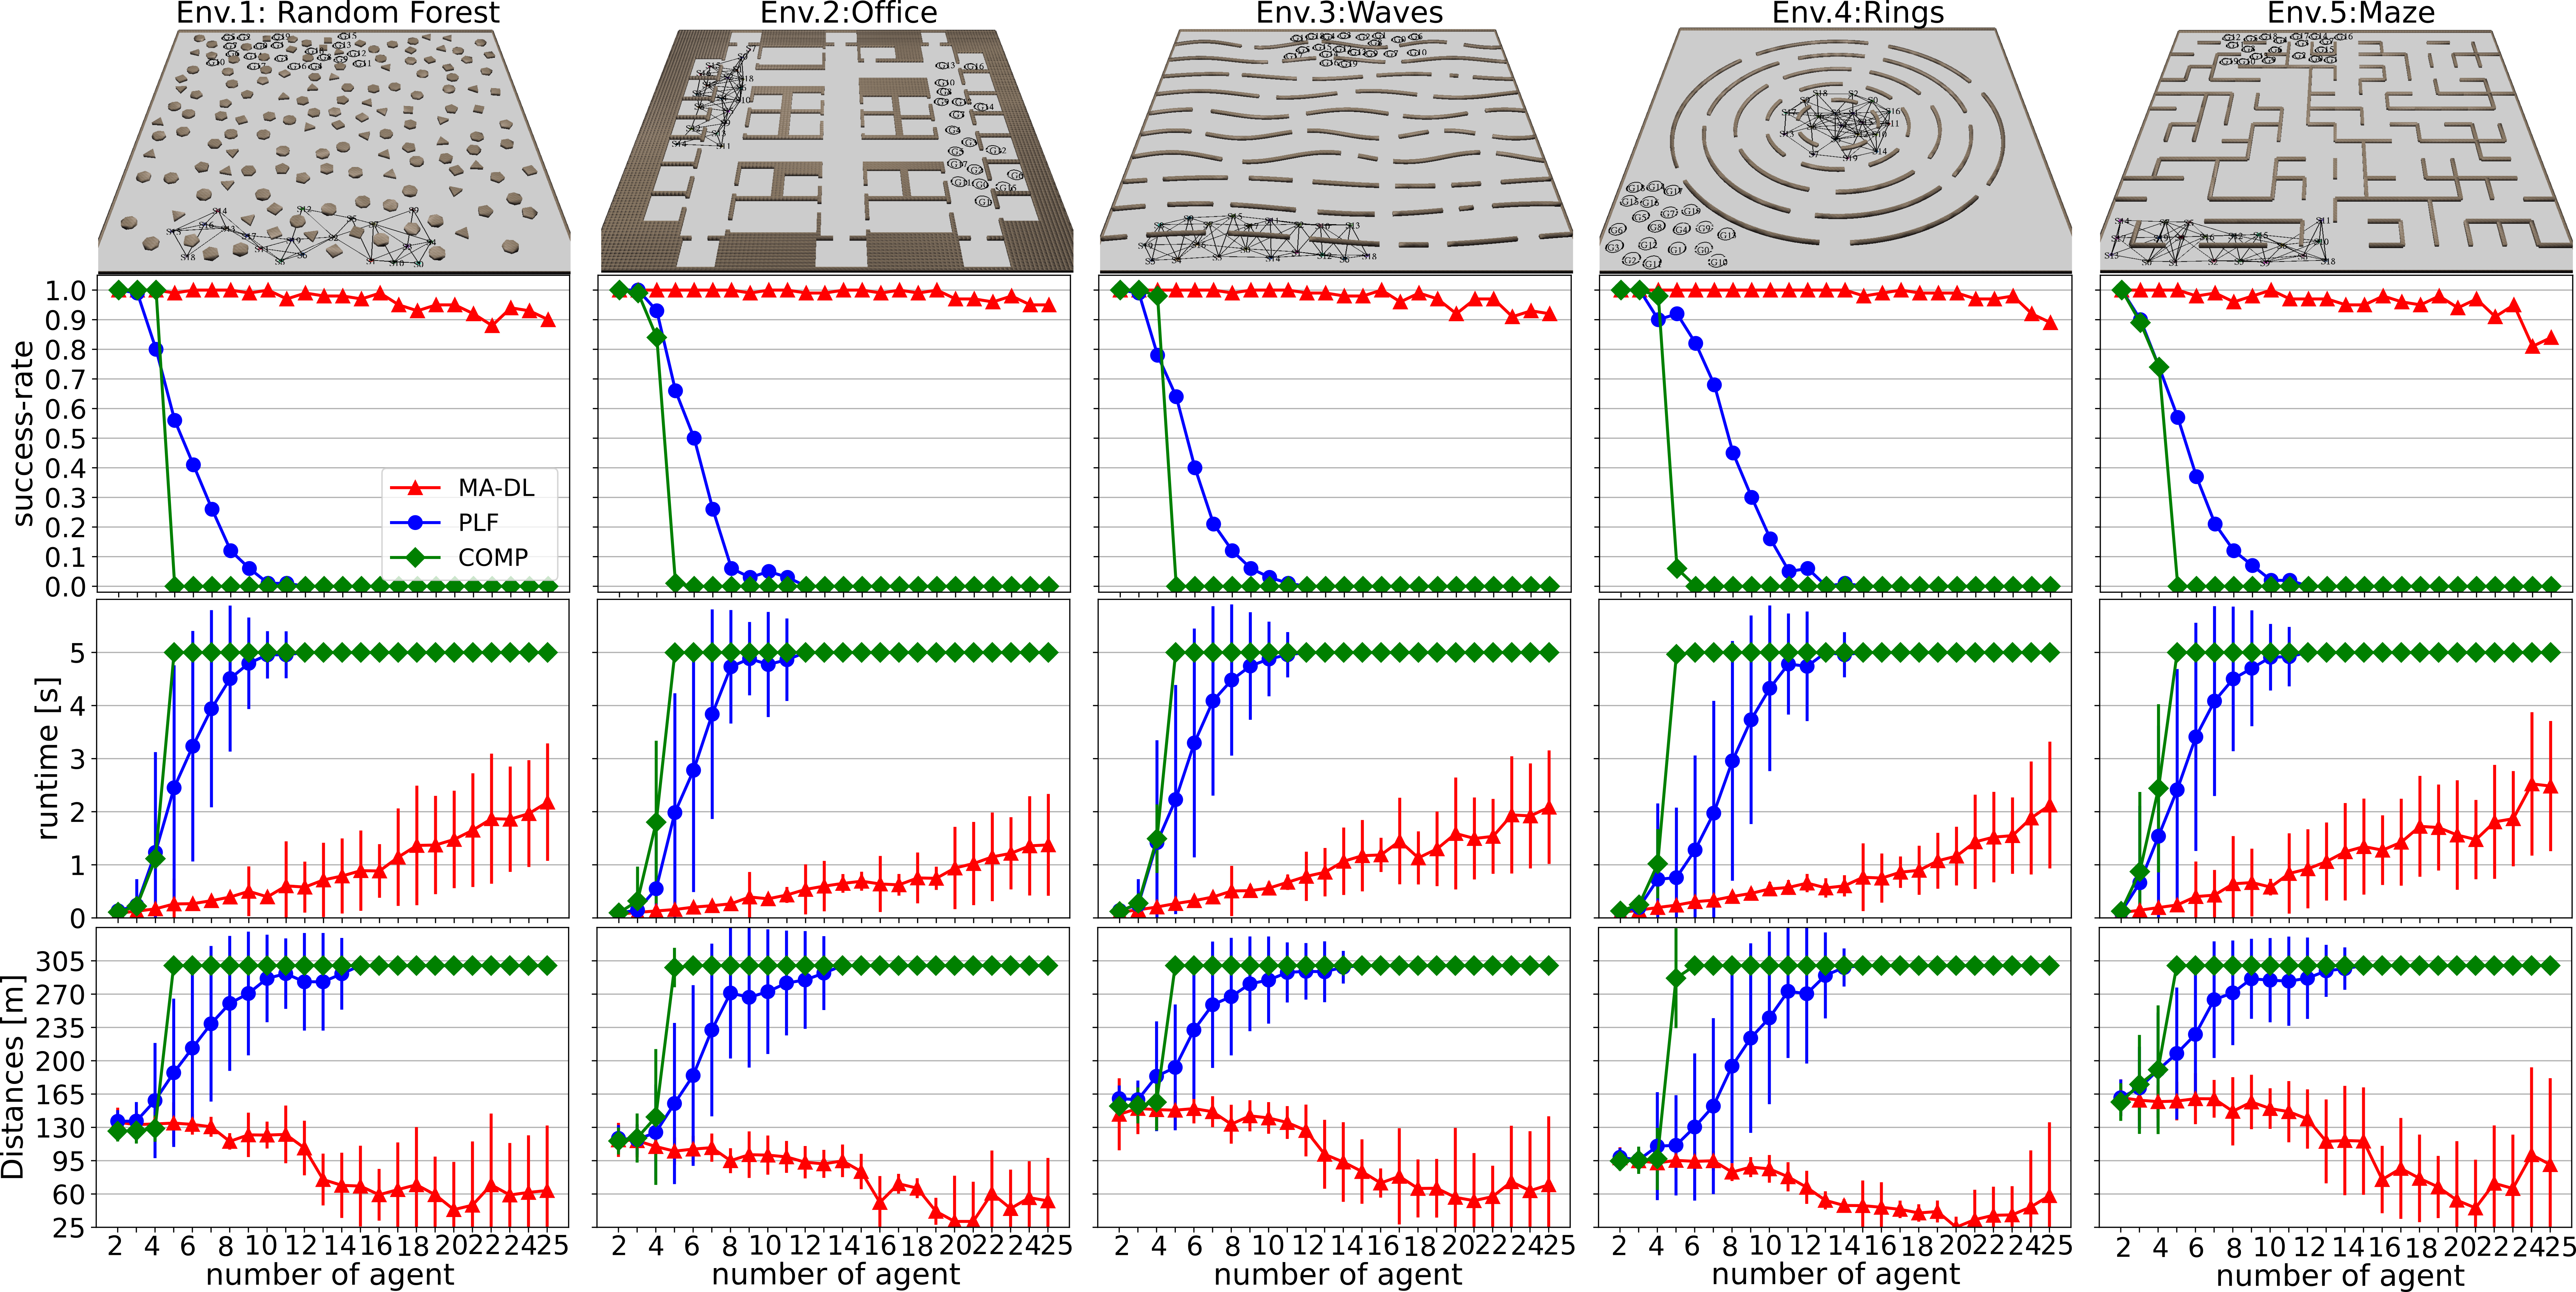
\includegraphics[width=1.0\textwidth]{agentNr_all_map.png}

\caption{\textbf{Success-rate, Runtime, and Travel Distances of MA-DL (ours), PLF, and COMP on 5 environment types}. The comm. range is 15 m and max-runtime is 5 s. The runtime and travel distances are shown by means and standard deviations.}
\label{fig:result-agentNr}
\end{figure*}

\subsection{Experimental Setup}

\subsubsection{Baselines} \label{exp:baselines}

We have implemented two baselines: Centralized approach with composite state (COMP) and Platooning Leader-Follower approach (PLF).
COMP is selected because existing MAPF planners—which typically advance the motion of each agent in isolation of one another and then attempt to resolve 
conflicts as necessary—are not well suited to handle the communication constraint, as the challenge of ensuring that all agents are in constant 
communication would require an undue number of repair operations, causing such planners to struggle (Section 2).
Meanwhile, PLF is chosen because it is a state-of-the-art approach to solve MALCR problem.

% In all experiments, agents have eight actions: South, North, East, West, and the diagonal moves. 
% The longer actions are segmented into smaller ones to check for communication constraint.
\begin{itemize}
    \item COMP grows a multi-agent tree via A* using informed by a heuristic of sum of shortest-to-goal paths from each agent.
    In joint-actions of single and diagonal moves, the diagonal ones are trimmed down to equal length with the single moves.
    \item PLF also builds a multi-agent tree and using priority 
    planning to grows the tree. At the root of tree expansion, the planning order is shuffled and so a 
    random leader is chosen; planning order is then fixed for downstream nodes.
    % The planner is allowed to revisit the root node during planning to propose alternate orderings.
    % As expanding the tree, if the selected node is the root, a new leader is selected randomly; then the corresponding planning order is determined. Both are passed to the children nodes.
    % Otherwise, the leader and planning order do not change.
    The followers plan to follow another agent if its preceding agent reached its goal.
    % The MATree is expanded after the single-agent plannings finish. 
    If the current expansion fails after some iterations, the planning starts again at the root with a 
    new random leader and corresponding planning order.
\end{itemize}


\subsubsection{Environments and Instances} 
We evaluate MA-DL in five obstacle-rich environment types: Random Forest, Office, Waves, Rings, and Maze 
(Fig.~\ref{fig:result-agentNr}). All environments are square shapes of size $114 \times 114 $ m. 
On each environment type, there are one hundred maps generated with random locations of obstacles.

For each number of agents, one instance is generated on each environment map. 
So, there are total of 12000 instances for the experiments. 
The start and goal configurations are chosen randomly on alternate sides of the maps (except the ring environment), distributed with a rectangular area. 
The configurations are satisfied the TCOMM constraint.
Communication between two agents are established if the distance between them is within 15 m of one another.

\paragraph{Env. Type 1: Random Forest} (Fig.~\ref{fig:result-agentNr}) Obstacles with random shapes and sizes are distributed randomly occupying 10\% of the environment's area.

\paragraph{Env. Type 2: Office} (Fig.~\ref{fig:result-agentNr}) The environments consists multiple rooms and hallways. The room has a fixed width and varying length from 9--13 m. There are three long hallways along the building, 2--3 short hallways connecting them. The hallway width varies from 7--9 m.   

\paragraph{Env. Type 3: Waves} (Fig.~\ref{fig:result-agentNr}) The environments have wave-like obstacles which are separated at regular distances. Gaps are placed in each wave with random widths. The number of waves is set to $10$.

\paragraph{Env. Type 4: Rings} (Fig.~\ref{fig:result-agentNr}) The environments are featured by concentric rings with six breaks of random widths within 6--8 m. The separation between the rings is set to 8 m. For each instance, the starts are randomly placed at the center, and the goals are on one of four corners of the maps.

\paragraph{Env. Type 5: Maze} (Fig.~\ref{fig:result-agentNr}) The environments consist of mazes generated by Kruskal's algorithm with size of $14 \times 14$. To ease in generation of the starting and goal configurations, boundary walls connecting to the top-most and bottom-most rows are removed.
% the maze's top-most and bottom-most walls are removed. to the upper and lower boundary walls are removed. 

\subsubsection{Measuring Performance} 
We evaluate our framework against COMP and PLF baselines on 100 instances for each environment type and number of agent, measuring success-rate, average runtime and average distance traveled per agent. 
Planning is considered successful if all agents reach their goals within 5 s of runtime. Runs that exceed that planning ceiling are assigned a travel distance of 300 m.
% Otherwise, the runtime is set to 5 s and travel distance to 300 m for each agent.
The framework is evaluated with variations over number of agents, goal configurations, runtime, and environment difficulty levels. 

\subsubsection{Computing Resources} 
The experiments ran on HOPPER, a computing cluster provided by GMU's Office of Research Computing. Each planning instance 
is run single threaded, yet experiment were run in parallel across 48 cores on a 2.40GHz processor. Our code was developed 
in C++ and compiled with g++-9.3.0.

% The experiments ran on HOPPER, a computing cluster provided by GMU's Office of Research Computing and 
% Each node has 48 cores with Dell PowerEdge R640 Intel(R) Xeon(R) Gold 6240R CPU 2.40GHz. 
% The experiments were parallelized on multiple cores. 


\subsection{Results}
% Experiments study performance of our approach with varying agent number, runtime, and environment difficulty.
% We implement the experiments on these environments with varying the numbers of agent, the runtime, and difficulty.

\subsubsection{Results when varying the agent number} 
We tested the MA-DL planner with 2--25 agents, allocating 5 seconds of runtime, and the results are shown in Fig.~\ref{fig:result-agentNr}. MA-DL performs well with up to 25 agents, achieving over 90\% success-rate in all environments except Maze Env. The long narrow passages of the maze mean that if some agents stop at the beginning of these passages, it becomes very difficult for others to pass through, leading to extended runtime for expanding the MATree.

Both baseline planners struggle as the number of agents is increased. PLF manages up to 5 agents in Rings Env. and only 3-4 agents in other environments. % due to increasing directional diversity between the followers and the leader.
The heuristic of shortest-to-goal path sum guides COMP well to handle up 4 agents in Random Forest, Rings, and Waves Env. However, with greater than 6 agents, the high dimensionality of the search space means that planning cannot reach the goal in the allotted time and success rate quickly declines.
% in environments with many non-convex obstacles such as Maze and Office Env., the heuristic gets difficulty to inform COMP , then deteriorates in Maze and Office Env. 
% which contain  Sum of shortest paths heuristic can guide the planner well with small number of agents and convex obstacles. However, as increasing number of agent in non-convex spaces, the heuristic gets difficulty to select the best node to expand. 

In addition to average success rate, we also report the mean and standard deviation for runtime and travel distance in Fig.~\ref{fig:result-agentNr}. If a planner fails, the runtime and traveled distance penalties are applied to the results. The runtime and distance results aligned with the success-rate results across all planners.

\subsubsection{Results when varying runtime}

In this experiment, we run the planners with various runtime from 1 s to 512 s. We select the Maze Env., the most challenging Env. type for the experiments. The results are shown in Fig.~\ref{fig:rt_envhardness}.a, showing that success-rate reaches 100\% as the runtime grows. 

\begin{figure}[tb]
\setlength{\tabcolsep}{1pt}
\centering
\begin{tabular}{cc}
    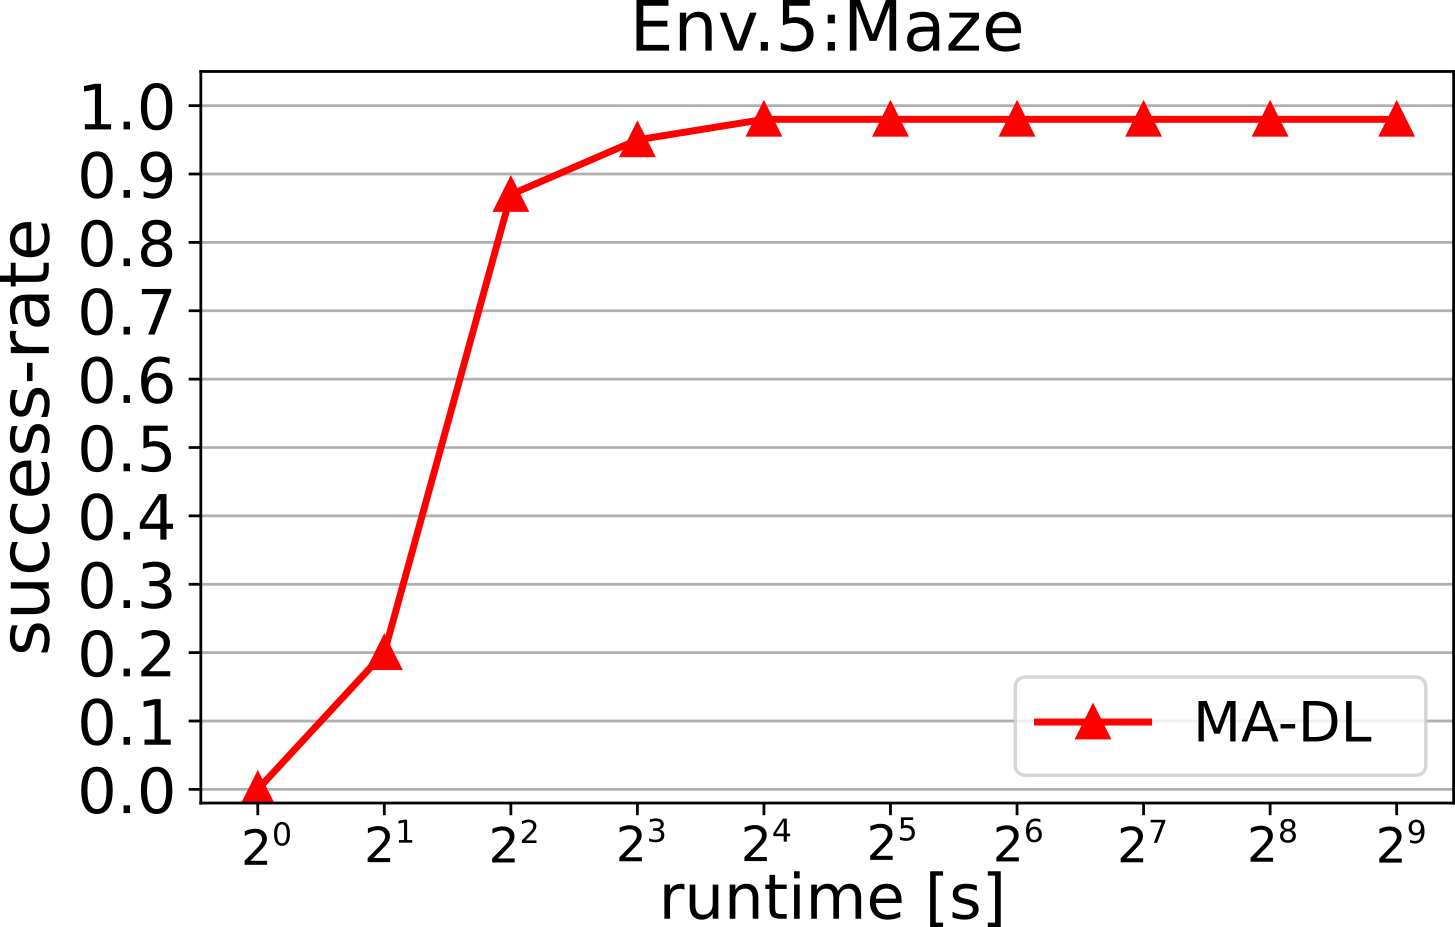
\includegraphics[width=0.193\textwidth]{timeVarying_23.png} &
    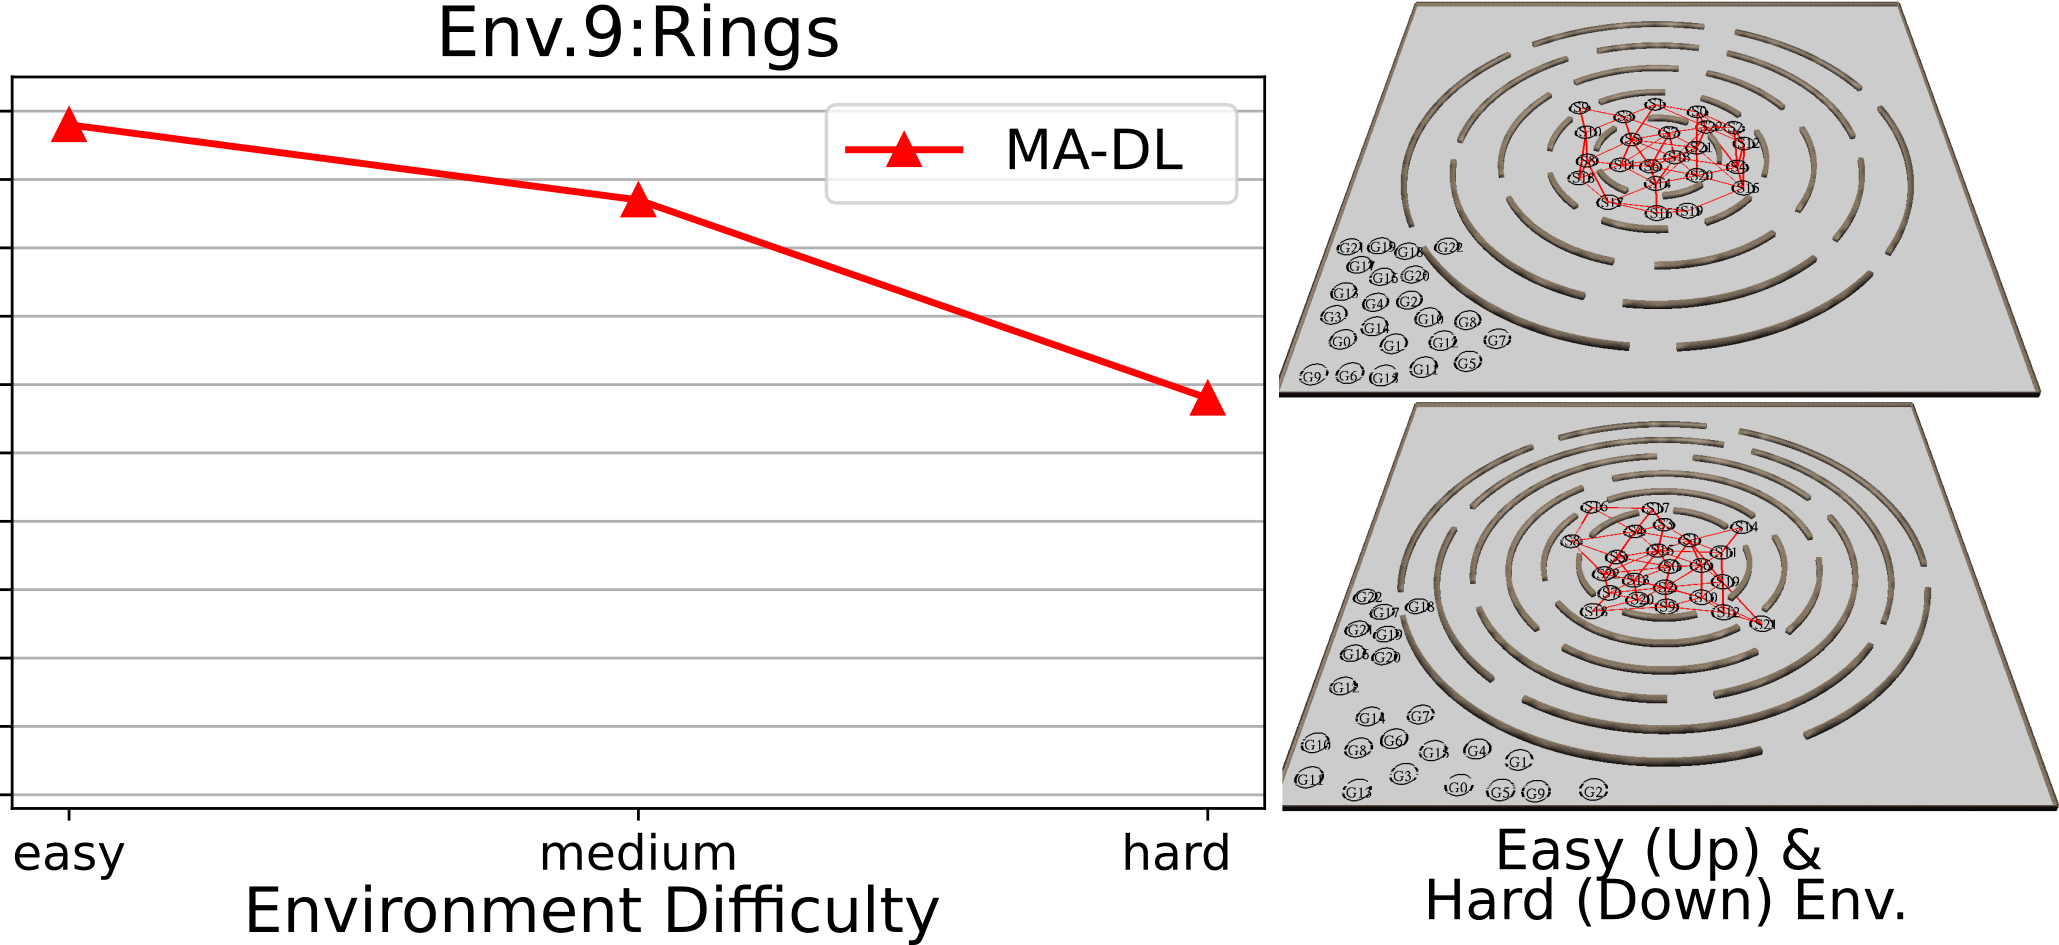
\includegraphics[width=0.275\textwidth]{envlevel_1.png} \\
    {\footnotesize{a) Success-rate vs Runtime}} &
    {\footnotesize{b) Success-rate vs Env. Difficulty}} 
\end{tabular}
\caption{\textbf{Performance of MA-DL as varying the runtime (a) and environment difficulty (b) with 23 agents}.}
\label{fig:rt_envhardness}
\end{figure}

% \begin{figure}[ht]
%         \centering
%         \begin{subfigure}[b]{0.35\linewidth}
%             \centering
%             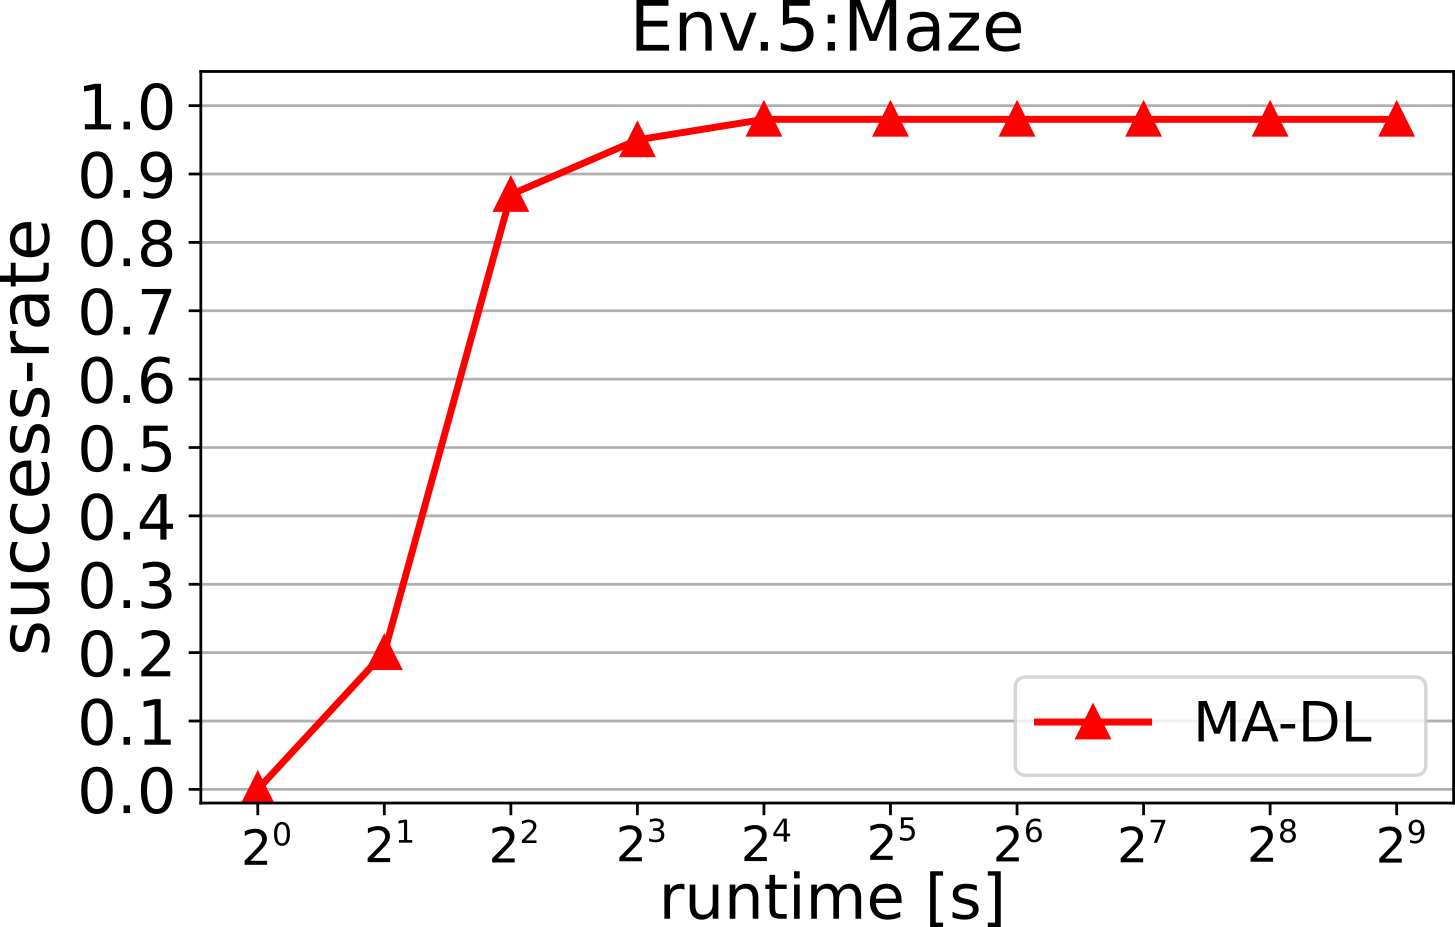
\includegraphics[width=1.0\linewidth]{timeVarying_23.png}
%             \caption{Success-rate vs Runtime}
%             \label{fig:image1}
%         \end{subfigure}
%         % \hfill
%         \begin{subfigure}[b]{0.5\linewidth}
%             \centering
%             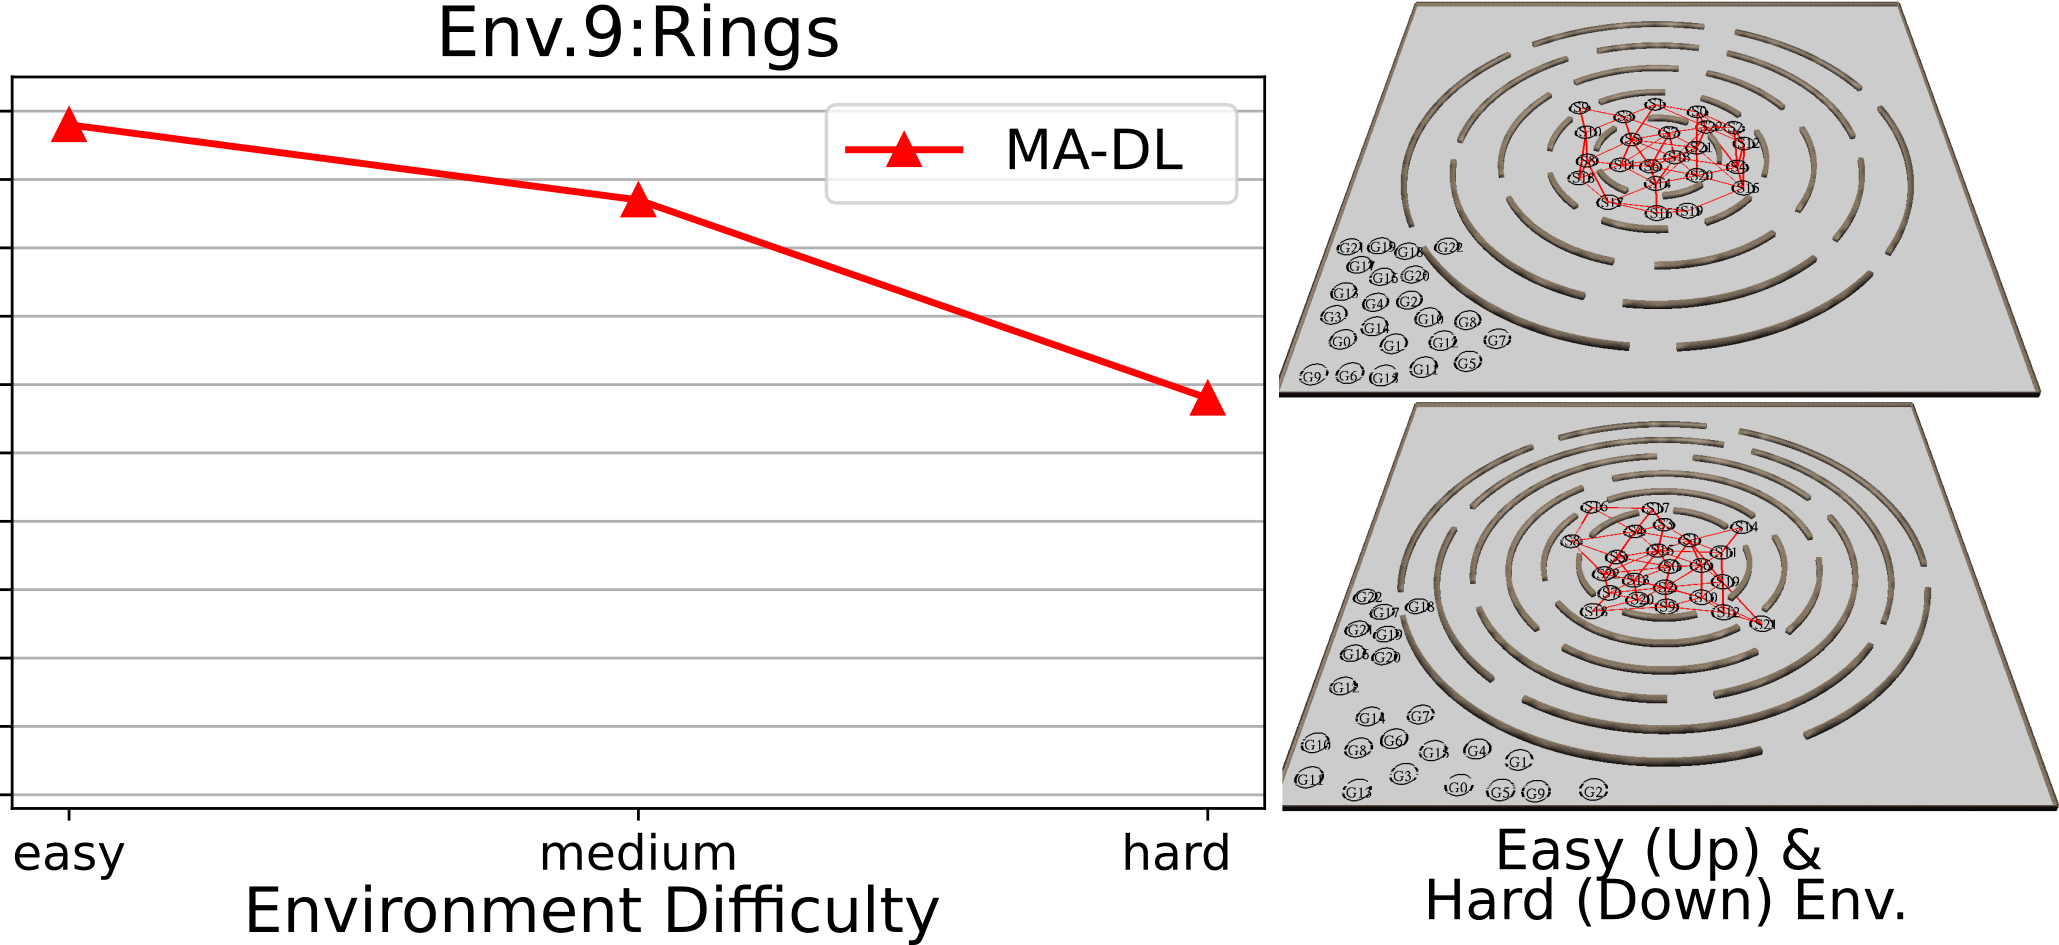
\includegraphics[width=1.0\linewidth]{envlevel_1.png}
%             \caption{Success-rate vs Env. Difficulty}
%             \label{fig:image2}
%         \end{subfigure}
%         \caption{Performance of MA-DL as varying the runtime (a) and environment difficulty (b) with 23 agents.}
%         \label{fig:rt_envhardness}
% \end{figure}


\subsubsection{Results when varying environment difficulty}

To demonstrate the robustness of our framework, we run MA-DL on variations of the Rings environment type with three difficulty levels: \textit{easy}, \textit{medium}, and \textit{hard}. The difficulty is controlled by the number of concentric rings, distance between consecutive rings, and number of breaks/gates on the rings. The features controlling difficulty are shown in Table~\ref{tab:hardnessEnvPara}. An easy and hard environment are shown in Fig.~\ref{fig:rt_envhardness}.b. 
\begin{table}[ht]
    \centering
    \begin{tabular}{c|c|c|c}
        \hline
         Diff. Level & Ring Count & Ring-Distance & Break Count \\
         \hline
         Easy & 4--5& 8.0 m & 6--7 \\
         \hline
         Medium & 5& 7.0 m & 5--6 \\
         \hline
         Hard & 6 & 5.5 m & 4--5\\
         \hline
    \end{tabular}
    \caption{Environment Difficulty Features}
    \label{tab:hardnessEnvPara}
\end{table}
 
The performances on three environment types with 23 agents and 5 s runtime are shown in Fig.~\ref{fig:rt_envhardness}.b with success-rate decreasing from easy to hard level. With medium or hard levels, MA-DL planner needs more than 5 s runtime to find valid paths for the agents.



\subsubsection{Results with Different Goal Configurations}

The goal configuration distribution impacts the planner's performance, especially when managing diverse agent movement. A thin, long goal distribution increases runtime as the planner must search longer for a suitable planning order. We run MA-DL with an alternate goal configuration distributions: long and thin versus rectangular (Fig.~\ref{fig:env-goaldist}) to test its robustness.
\textit{Following with ACOMM} makes the MA-DL robust in handling diverse movement directions across most environments (similar to Random Forest Env.-Fig.~\ref{fig:env-goaldist}.left). However, in Maze environments with narrow passages and only one way to go, frequent collisions and path modifications significantly increase difficulty of the planning problem, reducing planning performance somewhat.

\begin{figure}[bt]
\centering
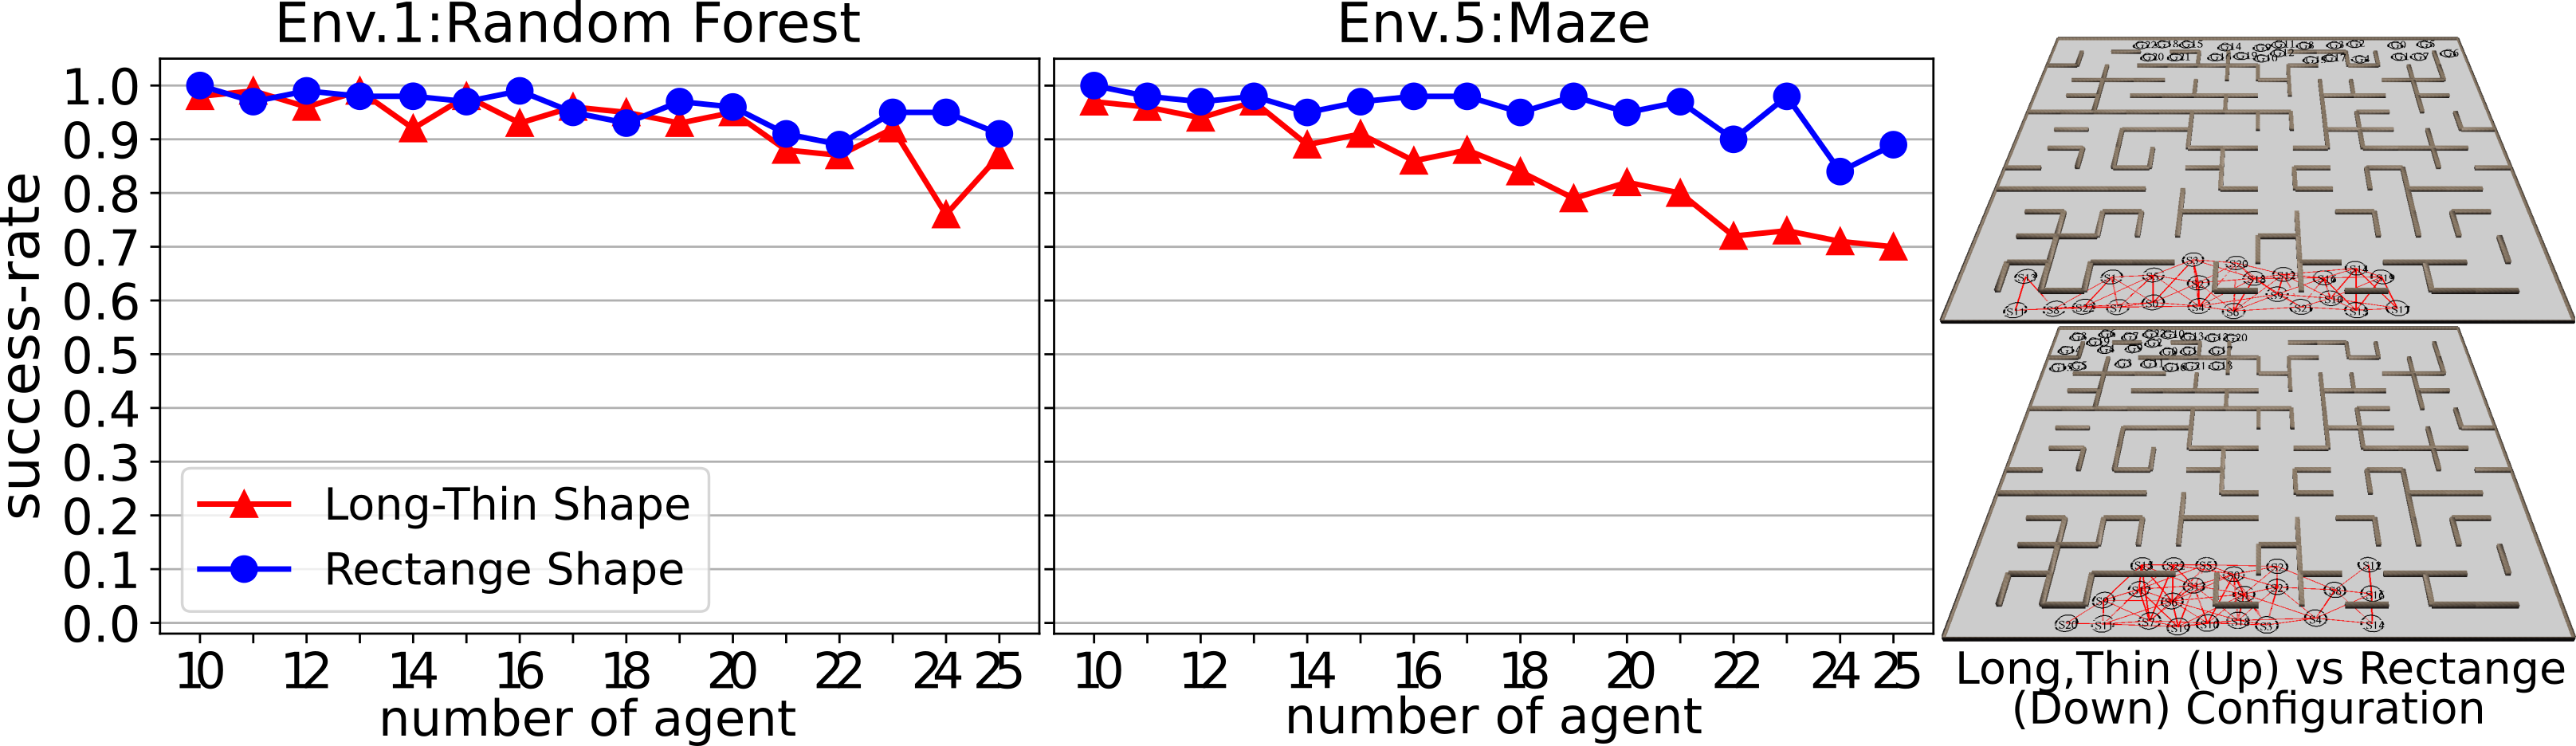
\includegraphics[scale=0.25]{goalDist.png}
\caption{\textbf{Long-Thin vs Rectangle of Goal Configuration.}}
\label{fig:env-goaldist}
\end{figure}

\section{Completeness Analysis}
Though our MA-DL planner represents an advance over leader-follower planners by overcoming a limitation of fixed-priority-order that results in their incompleteness, \textit{MA-DL is also incomplete in this domain}. We present an analysis of specifically what causes this incompleteness and present a direction to overcome this limitation for future work.

Ma et al.~\cite{ma2019searching} proved the following theorem for the incomplete prioritized planning:

\noindent{}\textbf{Theorem 1}: \textit{Prioritized (fixed) planning with an arbitrary priority ordering is incomplete for MAPF in general}.

\noindent{}Based on this theorem, fixed and platooning leader-follower approaches are incomplete planners. A fix leader-follower planner never changes the planning order, while a platooning planner only does so when members leave the team.
However, while our MA-DL planner overcomes this limitation, it is also an \textit{incomplete} algorithm. This is a consequence of the greedy nature of the single agent planner (SAPF), which always immediately returns upon finding a valid single agent path. We illustrate a scenario in Fig.~\ref{fig:complete_break} that MA-DL fails to solve: though the solution requires that agent $a_3$ select a longer path to allow other agents to pass by, the SAPF planner returns only the shortest path and so the team becomes stuck.
% , a longer The SAPF planner returns only the shortest path, leading all agents to pass through $G_1$, where they get stuck as $a_3$ reaches its goal. 

Future work could explore extending our MA-DL approach to achieve completeness. For this to be possible, the SAPF single-agent planner would need to be extended to eventually generate all possible paths when expanding each agent, a modification that would require careful consideration and detailed study so that it would not dramatically slow planning performance.
In this research, our focus is on developing a fast and practical planner that can efficiently handle the MALCR problem, outperforming existing approaches. We plan to develop a complete version of the MA-DL planner in the future research.

% To make the MA-DL planner complete, the single-agent planner must provide all possible paths from start to goal, allowing agents to explore alternatives, such as passing through $G_2$, to avoid congestion at $G_1$.

\begin{figure}
    \centering
    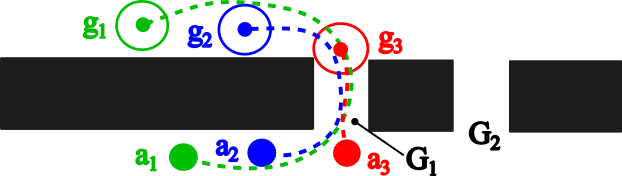
\includegraphics[width=0.7\linewidth]{complete_break.png}
    \caption{\textbf{A scenario demonstrating the incompleteness of MA-DL.} Due to the greedy nature of SAPF (find the shortest path), all agents attempt to go through $G_1$ without trying $G_2$ and cannot all reach their respective goals.}
    \label{fig:complete_break}
\end{figure}



\section{Conclusion} \label{sec:conclusion}

This paper introduces the MA-DL framework to handle the MALCR problem. The core advance 
of our approach is \textit{dynamic leading}, which enables the dynamic reselection of 
the leading agent during path planning whenever progress stalls, overcoming a key 
limitation of state-of-the-art platooning approaches.
% Additionally, following with ACOMM technique helps the planner resolve issues of heading different directions between leader and followers.
% We also developed a function to handle \textit{out-communication-at-goal} situations, significantly reducing the planning runtime.
We have tested our MA-DL planner in multiple environments with features such as 
obstacles-rich, narrow passages, non-convex spaces, and long hallways. The results 
demonstrate the robustness of MA-DL planner, capable of planning up to 25 agents within 
5 seconds of runtime.
In future work, we aim to develop a complete version of this planner. 
We also intend to design a new heuristic to improve the expansion of single agent trees.
Furthermore, we plan to extend the framework to support robot teams with rich kinodynamic 
constraints, bringing it a step closer to the real-world applications.









\addtolength{\textheight}{-12cm}   % This command serves to balance the column lengths
                                  % on the last page of the document manually. It shortens
                                  % the textheight of the last page by a suitable amount.
                                  % This command does not take effect until the next page
                                  % so it should come on the page before the last. Make
                                  % sure that you do not shorten the textheight too much.

%%%%%%%%%%%%%%%%%%%%%%%%%%%%%%%%%%%%%%%%%%%%%%%%%%%%%%%%%%%%%%%%%%%%%%%%%%%%%%%%



%%%%%%%%%%%%%%%%%%%%%%%%%%%%%%%%%%%%%%%%%%%%%%%%%%%%%%%%%%%%%%%%%%%%%%%%%%%%%%%%



%%%%%%%%%%%%%%%%%%%%%%%%%%%%%%%%%%%%%%%%%%%%%%%%%%%%%%%%%%%%%%%%%%%%%%%%%%%%%%%%
\section*{ACKNOWLEDGMENT}

The work by E. Plaku is supported by (while serving at) the National Science Foundation. 
Any opinion, findings, and conclusions or recommendations expressed in this material are 
those of the authors, and do not necessarily reflect the views of the National Science 
Foundation.

This material is based upon work supported by the National Science Foundation under Grant 
No. 2232733. G. J. Stein acknowledges support from this grant.

% \bibliography{refs.bib}
\bibliography{IEEE_madl.bib}
\bibliographystyle{IEEEtran}


%%%%%%%%%%%%%%%%%%%%%%%%%%%%%%%%%%%%%%%%%%%%%%%%%%%%%%%%%%%%%%%%%%%%%%%%%%%%%%%%



\end{document}
